% !TEX root = main.tex

\newchapter{Analytische Lösung Aufgabe 1}{}
Aufgrund der vorteilhaften Struktur des Problems der ersten Aufgabenstellung (elektrostatische Simulation) ist eine analytische Lösung möglich. Mit dieser kann darauffolgend das Ergebnis der numerischen Simulation überprüft und plausibilisiert werden. \\ \\
Wie die folgende Rechnung zeigen wird, kann das Ergebnis der analytischen Rechnung ebenso wieder nur approximiert dargestellt werden, da im Resultat eine unendliche Summe auftaucht. Nichtsdestotrotz ist aufgrund moderne numerischer Rechenprogramme eine Auswertung des Ergebnisses mit hinreichender Genauigkeit möglich. 

\newsection{Formulierung des Problems}{}
Für die analytische Rechung wird die sogenannte Separationsmethode zur Lösung der Laplaceschen Gleichung herangezogen.
\begin{align}
	\label{eq:LaplaceV_ana}
	\Delta V = \pDiffDiff{V}{x} + \pDiffDiff{V}{y} + \pDiffDiff{V}{z}
\end{align}

Aufgrund der Ausdehung des Problems in z-Richtung ($L << L_A$) kann die ursprüngliche dreidimensionale Aufgabenstellung in zwei Dimensionen betrachtet werden, da näherungsweise keine Änderung des Potentials in z-Richtung auftritt. 
\begin{align}
\label{eq:LaplaceVz_ana}
	\pDiffDiff{V}{z} = 0
\end{align}

Damit ergibt sich folgendes zu lösendes Randwertproblem, wie auch bereits in Gleichung~\ref{eq:Randwertproblem_simple} angeführt:
\begin{align}
	\label{eq:Randwertproblem_simple_ana}
	&\pDiffDiff{V}{x} + \pDiffDiff{V}{y} = 0 \text{ mit }\\
	&V = V_D \text{ auf } \Gamma_D \nonumber\\
	&\pDiff{V}{n} = 0 \text{ auf } \Gamma_N \nonumber
\end{align}

Eine Neumann'sche Randbedindung (auf $\Gamma_N$) ist laut Aufgabenstellung nicht gegeben. Die Dirichlet'schen Randbedingungen (auf $\Gamma_D$) ergeben sich durch die Vorgabe der Potentiale der vier Metallplatten. 

\newsection{Separationsmethode}{}
Bei dieser Methode zur Lösung von partiellen Differentialgleichungen wird versucht, die Laplace'sche Gleichung für $V$ auf gewöhnliche Differentialgleichungen zurückzuführen. Hierbei wählt man als Ansatz für die Potentialfunktion ein Produkt der Lösungen dieser gewöhnlichen Differentialgleichungen, welche ausschließlich von einer Ortskoordinate abhängen. 
\begin{align}
	\label{eq:Separationsmethode_3D}
	V_{(x,y,z)} = X_{(x)} \cdot Y_{(y)} \cdot Z_{(z)}
\end{align}

Aufgrund der räumlichen Ausdehnung in z-Richtung ergibt sich, wie in Gleichung~\ref{eq:Randwertproblem_simple_ana} angeführt:
\begin{align}
	\label{eq:Separationsmethode_2D}
	V_{(x,y)} = X_{(x)} \cdot Y_{(y)}
\end{align}

Damit die Separationsmethode angewandt werden kann, müssen die Randbedingungen entlang Oberflächen mit $x = konst.$ und $y = konst.$ gegeben sein. Dies ist hier der Fall, denn die erwähnten Oberflächen entsprechen genau den Metallplatten, auf welchen die Dirichlet'schen Randbedingungen gegeben sind. \\

\newsection{Ableitung der Potentialfunktion}{}
Einsetzen von Gleichung~\ref{eq:Separationsmethode_2D} in die Laplace'sche Gleichung~\ref{eq:LaplaceV_ana} und anschließendem Umformen führt zu:
\begin{align}
	\label{eq:Sep_Ableitung1}
	&Y_{(y)} \dfrac{\mathrm{d}^2 X_{(x)}}{\mathrm{d}x^2} + X_{(x)} \dfrac{\mathrm{d}^2 Y_{(y)}}{\mathrm{d}y^2} = 0 \qquad | :X_{(x)} Y_{(y)} \\
	&\underbrace{\frac{1}{X_{(x)}} \dfrac{\mathrm{d}^2 X_{(x)}}{\mathrm{d}x^2}}_{\underbrace{f_{(x)}}_{k^2}} + \underbrace{\frac{1}{Y_{(y)}} \dfrac{\mathrm{d}^2 Y_{(y)}}{\mathrm{d}y^2}}_{\underbrace{g_{(y)}}_{-k^2}} = 0 \label{eq:Sep_Ableitung2}
\end{align}

Die beiden Summanden aus Gleichung~\ref{eq:Sep_Ableitung2} hängen also nur mehr von jeweils einer Variable ab und werden zu einer Konstanten mit jeweils einmal positivem und einmal negativem Vorzeichen gesetzt, womit die Forderung $=0$ erfüllt wird. Damit hat sich das Problem auf zwei gewöhnliche Differentialgleichungen reduziert, welche mit der Ansatzmethode gelöst werden können. 

\begin{align}
	&\dfrac{\mathrm{d}^2 X_{(x)}}{\mathrm{d}x^2} = k^2 X_{(x)} \\
	&\mathrm{Ansatz:}~X_{(x)} = \e^{\lambda x} \\
	&\Rightarrow \lambda^2 \e^{\lambda x} = k^2 \e^{\lambda x} \\
	&\Rightarrow \lambda^2 - k^2 = 0 \\
	&\lambda_{1,2} = \pm \sqrt{k^2} = \pm k \\
	&\Rightarrow X_{(x)} = \tilde{A} \e^{kx} + \tilde{B} \e^{-kx}
\end{align}

Der Ausdruck für $X_{(x)}$ kann mit Hilfe der Hyperbelfunktionen umgeschrieben werden:
\begin{align}
	 X_{(x)} = A\cosh(kx) + B\sinh(kx)
\end{align}

Das selbe Vorgehen wendet man nun für $g_{(y)}$ an. 
\begin{align}
	&\dfrac{\mathrm{d}^2 Y_{(y)}}{\mathrm{d}y^2} = -k^2 Y_{(y)} \\
	&\mathrm{Ansatz:}~Y_{(y)} = \e^{\lambda y}  \notag \\
	&\Rightarrow \lambda^2 \e^{\lambda y} = -k^2 \e^{\lambda y}  \notag \\
	&\Rightarrow \lambda^2 + k^2 = 0  \notag \\
	&\lambda_{1,2} = \pm \sqrt{-k^2} = \pm jk  \notag  \\
	&\Rightarrow Y_{(y)} = \tilde{C} \e^{jky} + \tilde{D} \e^{-jky}
\end{align}

Der Ausdruck für $Y_{(y)}$ kann mit Hilfe der trigonometrischen Funktionen umgeschrieben werden:
\begin{align}
	 Y_{(y)} = C\cos(ky) + D\sin(ky)
\end{align}

Setzt man nun beide Ausdrücke gemäß Gleichung~\ref{eq:Separationsmethode_2D} zusammen, erhält man:
\begin{align}
	\label{eq:Sep_V1}	
	V_{(x,y)} = \bigl[A\cosh(kx) + B\sinh(kx)\bigr] \cdot \bigl[C\cos(ky) + D\sin(ky)\bigr]
\end{align}

Vertauscht man in Gleichung~\ref{eq:Sep_Ableitung2} die beiden Vorzeichen der Konstante $k$, also $f_{(x)} = -k^2$ und $g_{(y)} = k^2$, anstatt $f_{(x)} = k^2$ und $g_{(y)} = -k^2$, so kann man mit selben Vorgehen wie oben folgenden Ausdruck für $V$ ableiten:
\begin{align}
	\label{eq:Sep_V2}	
	V_{(x,y)} = \bigl[A\cos(kx) + B\sin(kx)\bigr] \cdot \bigl[C\cosh(ky) + D\sinh(ky)\bigr]
\end{align}

Hier sind also $\cos$ mit $\cosh$ und $sin$ mit $sinh$ vertauscht. Im folgenden werden beide Ansätze notwendig sein, damit der sogenannte \glqq Fouriertrick\grqq{} korrekt angewandt werden kann. Hierzu ist es nämlich notwendig, dass jene Variable, welche im \glqq Fouriertrick\grqq{} als Integrationsvariable dient, in den trigonometrischen Funktionen vorkommt, da nur diese bei der Integration wegfallen. 

\newsection{Superpositionsprinzip}{}
Aufgrund der Linearität der Laplace'schen Gleichung kann das Superpositionsprinzip angewandt werden. In der Aufgabenstellung ist das Potential von vier Metallplatten vorgegeben, ergo ergeben sich vier Dirichlet'sche Ränder bzw. Randbedingungen. Das Superpositionsprinzip erlaubt es nun, das Problem in vier Teilprobleme zu zerlegen, in welchen jeweils nur eine Dirichlet'sche Randbedingung aktiv ist und die restlichen sozusagen \glqq ausgeschalten\grqq{} beziehungsweise zu $0$ gesetzt sind. Die Betrachtung in Teilproblemen vereinfacht die Berechnung der jeweiligen Teillösungen, welche gemäß des Superpositionsprinzips anschließend additiv überlagert werden müssen, um die Gesamtlösung der Potentialverteilung zu erhalten, welche gilt, wenn alle Randbedingungen aktiv sind. 

\newsection{Berechnung der Teillösungen}{}
\newsubsection{Potential A aktiv}{}
Da das Potential $V_A$ über einen Bereich mit $y = 0 = konstant$ wirkt, muss der Ansatz aus Gleichung~\ref{eq:Sep_V2} verwendet werden. 
\begin{align}
	V_{(x,y)} = \bigl[A\cos(kx) + B\sin(kx)\bigr] \cdot \bigl[C\cosh(ky) + D\sinh(ky)\bigr]
\end{align}

Mit den Randbedingungen können nun die jeweiligen Koeffizienten der Teillösung berechnet werden. 

\begin{enumerate}
	\item \begin{align}
		&V_{(0,y)} = V_D = 0 = A \cdot \bigl[C \cosh(ky) + D \sinh(ky)\bigr] \\
		&\Rightarrow A = 0  \notag 
	\end{align}
	\begin{align}
		V_{(x,y)} = \bigl[\bar{C} \cosh(ky) + \bar{D} \sinh(ky)\bigr] \cdot \sin(kx)
	\end{align}
	
	\item \begin{align}
		&V_{(L,y)} = V_B = 0 = \bigl[\bar{C} \cosh(ky) + \bar{D} \sinh(ky)\bigr] \cdot \sin(kL) \\
		&\Rightarrow kL = n \pi \notag \\   
		&\Rightarrow k = n \frac{\pi}{L}  \notag 
	\end{align}
	Da diese Bedingung für beliebiges $n \in \mathbb{N}$ gilt, müssen diese in der Teillösung auch berücksichtigt werden. 
	
	\begin{align}
		V_{(x,y)} = \sum_{n = 1}^{\infty} \bigl[\bar{C}_n \cosh(n \frac{\pi}{L} y) + \bar{D}_n \sinh(n \frac{\pi}{L} y) \bigr] \cdot \sin(n \frac{\pi}{L} x)
	\end{align}
	
	\item \begin{align}
		V_{(x,0)} = V_A = \sum_{n = 1}^{\infty} \bar{C}_n \sin(n \frac{\pi}{L} x)
	\end{align}
	Die Koeffizienten $\bar{C}_n$ können nun mittels \glqq Fouriertrick\grqq{} bestimmt werden. 
	\begin{align}
		\bar{C}_n &= \frac{2}{L} \int_{0}^{L} V_A \sin(n \frac{\pi}{L} x) \mathrm{d}x \\
		&= - \frac{2V_A}{L} \frac{L}{n \pi} \cos(n \frac{\pi}{L} x) |_0^L \notag \\
		&= \frac{2V_A}{n \pi} \bigl[ 1 - \cos(n \pi) \bigr] \notag \\
		&= \biggl\{ \begin{matrix}
			0 \qquad \quad, n~\mathrm{gerade} \\
			~~~\frac{4V_A}{n \pi} \qquad , n~\mathrm{ungerade}
		\end{matrix} \notag
	\end{align}
	\begin{align}
		V_{(x,y)} = \sum_{n = 1,3,5,...} \biggl[ \frac{4V_A}{n \pi} \cosh(n \frac{\pi}{L} y) + \bar{D}_n \sinh(n \frac{\pi}{L} y) \biggr] \cdot \sin(n \frac{\pi}{L} x)
	\end{align}
	
	\item \begin{align}
		&V_{(x,L)} = V_C = 0 = \sum_{n = 1,3,5,...} \biggl[ \frac{4V_A}{n \pi} \cosh(n \pi) + \bar{D}_n \sinh(n \pi) \biggr] \cdot \sin(n \frac{\pi}{L} x) \\
		&\iff \bar{D}_n = - \frac{4V_A}{n \pi} \frac{\cosh(n \pi)}{\sinh(n \pi)} \notag
	\end{align}
	Da nun alle Koeffizienten bestimmt sind, kann folgender Ausdruck angegeben werden:
	
	\begin{align}
		V_{(x,y)} &= \sum_{n = 1,3,5,...} \frac{4V_A}{n \pi} \biggl[\cosh(n \frac{\pi}{L} y) - \frac{\cosh(n \pi)}{\sinh(n \pi)} \sinh(n \frac{\pi}{L} y) \biggr] \cdot \sin(n \frac{\pi}{L} x) \\
		&= \sum_{n = 1,3,5,...} \frac{4V_A}{n \pi} \biggl[\cosh(n \frac{\pi}{L} y) \sinh(n \pi) - \sinh(n \frac{\pi}{L} y) \cosh(n \pi) \biggr] \cdot \frac{\sin(n \frac{\pi}{L} x)}{\sinh(n \pi)} \notag
	\end{align}
\end{enumerate}

Um den Ausdruck in Gleichung~\ref{eq:V_Teil1_1} weiter zu vereinfachen, wird folgendes Additionstheorem verwendet:
\begin{align}
	\sinh(x \pm y) = \sinh(x)\cosh(y) \pm \cosh(x)\sinh(y)
\end{align}

Damit lässt sich nun die erste Teillösung für den Fall Potential $V_A$ aktiv anschreiben:

\begin{align}
	V_{(x,y)} &= \sum_{n = 1,3,5,...} \frac{4V_A}{n \pi} \frac{\sinh(n \pi - n \frac{\pi}{L} y)}{\sinh(n \pi)} \sin(n \frac{\pi}{L} x) \\
	&= \sum_{n = 1,3,5,...} \frac{4V_A}{n \pi} \frac{\sinh \bigl(n \pi (1 - \frac{y}{L})\bigr)}{\sinh(n \pi)} \sin(n \frac{\pi}{L} x) \notag \\
	&= \sum_{n = 1,3,5,...} \frac{4V_A}{n \pi} \frac{\sinh \bigl(n \pi \frac{L-y}{L}\bigr)}{\sinh(n \pi)} \sin(n \frac{\pi}{L} x) \label{eq:V_Teil1_1} \notag
\end{align}

\newsubsection{Potential B aktiv}{}
Da das Potential $V_B$ über einen Bereich mit $x = L = konstant$ wirkt, muss der Ansatz aus Gleichung~\ref{eq:Sep_V1} verwendet werden. 
\begin{align}
	V_{(x,y)} = \bigl[A\cosh(kx) + B\sinh(kx)\bigr] \cdot \bigl[C\cos(ky) + D\sin(ky)\bigr]
\end{align}

Mit den Randbedingungen können nun die jeweiligen Koeffizienten der Teillösung berechnet werden. 

\begin{enumerate}
	\item \begin{align}
		&V_{(x,0)} = V_A = 0 = \bigl[A \cosh(kx) + B \sinh(kx) \bigr] \cdot C \\
		&\Rightarrow C = 0 \notag
	\end{align}
	\begin{align}
		V_{(x,y)} = \bigl[ \bar{A} \cosh(kx) + \bar{B} \sinh(kx) \bigr] \cdot \sin(ky)
	\end{align}
	
	\item \begin{align}
		&V_{(0,y)} = V_D = 0 = \bar{A} \sin(ky) \\
		&\Rightarrow \bar{A} = 0 \notag
	\end{align}
	\begin{align}
		V_{(x,y)} = \bar{B} \sinh(kx) \sin(ky)
	\end{align}
	
	\item \begin{align}
		&V_{(x,L)} = V_C = 0 = \bar{B} \sinh(kx) \sin(kL) \\
		&\Rightarrow kL = n\pi \notag \\
		&\Rightarrow k = n \frac{\pi}{L} \notag
	\end{align}
	Da diese Bedingung für beliebiges $n \in \mathbb{N}$ gilt, müssen diese in der Teillösung auch berücksichtigt werden. 
	\begin{align}
		V_{(x,y)} = \sum_{n=1}^\infty \bar{B}_n \sinh(n \frac{\pi}{L}x) \sin(n \frac{\pi}{L}y)
	\end{align}
	
	\item \begin{align}
		V_{(L,y)} = V_B = \sum_{n=1}^\infty \bar{B}_n \sinh(n \pi) \sin(n \frac{\pi}{L}y)
	\end{align}
	Die Koeffizienten $\bar{B}_n$ können nun mittels \glqq Fouriertrick\grqq{} bestimmt werden. 
	\begin{align}
		\bar{B}_n &= \frac{2}{L} \frac{1}{\sinh(n \pi)} \int_0^L V_B \sin(n \frac{\pi}{L}y) \mathrm{d}y \\
		&= -\frac{2}{L} \frac{1}{\sinh(n \pi)} \frac{L}{n \pi} V_B \cos(n \frac{\pi}{L}y) |_0^L \notag \\
		&= \frac{2V_B}{n \pi} \frac{1}{\sinh(n \pi)} \bigl(1 - \cos(n \pi)\big) \notag \\
		&= \biggl\{ \begin{matrix}
			0 \qquad \qquad \quad , n~\mathrm{gerade} \\
			\frac{4V_B}{n \pi} \frac{1}{\sinh(n \pi)} \qquad , n~\mathrm{ungerade}
		\end{matrix} \notag
	\end{align}
	Da damit alle Koeffizienten bestimmt sind, lässt sich nun die zweite Teillösung für den Fall Potential $V_B$ aktiv anschreiben:
	\begin{align}
		V_{(x,y)} = \sum_{n = 1,3,5,...} \frac{4V_B}{n \pi} \frac{\sinh(n \frac{\pi}{L}x)}{\sinh(n \pi)} \sin(n \frac{\pi}{L}y) \label{eq:V_Teil1_2}
	\end{align}
\end{enumerate}

\newsubsection{Potential C aktiv}{}
Da das Potential $V_C$ über einen Bereich mit $y = L = konstant$ wirkt, muss der Ansatz aus Gleichung~\ref{eq:Sep_V2} verwendet werden. 
\begin{align}
	V_{(x,y)} = \bigl[A\cos(kx) + B\sin(kx)\bigr] \cdot \bigl[C\cosh(ky) + D\sinh(ky)\bigr]
\end{align}

Mit den Randbedingungen können nun die jeweiligen Koeffizienten der Teillösung berechnet werden. 

\begin{enumerate}
	\item \begin{align}
		&V_{(x,0)} = V_A = 0 = \bigl[A \cos(kx) + B \sin(kx) \bigr] \cdot C \\
		&\Rightarrow C = 0 \notag
	\end{align}
	\begin{align}
		V_{(x,y)} = \bigl[ \bar{A} \cos(kx) + \bar{B} \sin(kx) \bigr] \cdot \sinh(ky)
	\end{align}
	
	\item \begin{align}
		&V_{(0,y)} = V_D = 0 = \bar{A} \sinh(ky) \\
		&\Rightarrow \bar{A} = 0 \notag
	\end{align}
	\begin{align}
		V_{(x,y)} = \bar{B} \sin(kx) \sinh(ky)
	\end{align}
	
	\item \begin{align}
		&V_{(L,y)} = V_B = 0 = \bar{B} \sin(kL) \sinh(ky) \\
		&\Rightarrow kL = n\pi \notag \\
		&\Rightarrow k = n \frac{\pi}{L} \notag	
	\end{align}
	Da diese Bedingung für beliebiges $n \in \mathbb{N}$ gilt, müssen diese in der Teillösung auch berücksichtigt werden. 
	\begin{align}
		V_{(x,y)} = \sum_{n=1}^\infty \bar{B}_n \sin(n \frac{\pi}{L}x) \sinh(n \frac{\pi}{L}y)
	\end{align}
	
	\item \begin{align}
		V_{(x,L)} = V_C = \sum_{n=1}^\infty \bar{B}_n \sin(n \frac{\pi}{L}x) \sinh(n \pi)
	\end{align}
	Die Koeffizienten $\bar{B}_n$ können nun mittels \glqq Fouriertrick\grqq{} bestimmt werden. 
	\begin{align}
		\bar{B}_n &= \frac{2}{L} \frac{1}{\sinh(n \pi)} \int_0^L V_C \sin(n \frac{\pi}{L}x) \mathrm{d}x \\
		&= -\frac{2}{L} \frac{1}{\sinh(n \pi)} \frac{L}{n \pi} V_C \cos(n \frac{\pi}{L}x) |_0^L \notag \\
		&= \frac{2V_C}{n \pi} \frac{1}{\sinh(n \pi)} \bigl(1 - \cos(n \pi)\big) \notag \\
		&= \biggl\{ \begin{matrix}
			0 \qquad \qquad \quad , n~\mathrm{gerade} \\
			\frac{4V_C}{n \pi} \frac{1}{\sinh(n \pi)} \qquad , n~\mathrm{ungerade}
		\end{matrix} \notag
	\end{align}
	Da damit alle Koeffizienten bestimmt sind, lässt sich nun die dritte Teillösung für den Fall Potential $V_C$ aktiv anschreiben:
	\begin{align}
		V_{(x,y)} = \sum_{n = 1,3,5,...} \frac{4V_C}{n \pi} \frac{\sinh(n \frac{\pi}{L}y)}{\sinh(n \pi)} \sin(n \frac{\pi}{L}x) \label{eq:V_Teil1_3}
	\end{align}
\end{enumerate}

\newsubsection{Potential D aktiv}{}
Da das Potential $V_D$ über einen Bereich mit $x = 0 = konstant$ wirkt, muss der Ansatz aus Gleichung~\ref{eq:Sep_V1} verwendet werden. 
\begin{align}
	V_{(x,y)} = \bigl[A\cosh(kx) + B\sinh(kx)\bigr] \cdot \bigl[C\cos(ky) + D\sin(ky)\bigr]
\end{align}

Mit den Randbedingungen können nun die jeweiligen Koeffizienten der Teillösung berechnet werden. 

\begin{enumerate}
	\item \begin{align}
		&V_{(x,0)} = V_A = 0 = C \cdot \bigl[A \cosh(kx) + B \sinh(kx)\bigr] \\
		&\Rightarrow C = 0 \notag
	\end{align}
	\begin{align}
		V_{(x,y)} = \bigl[\bar{A} \cosh(kx) + \bar{B} \sinh(kx)\bigr] \cdot \sin(ky)
	\end{align}
	
	\item \begin{align}
		&V_{(x,L)} = V_C = 0 = \bigl[\bar{A} \cosh(kx) + \bar{B} \sinh(kx)\bigr] \cdot \sin(kL) \\
		&\Rightarrow kL = n \pi \notag \\
		&\Rightarrow k = n \frac{\pi}{L} \notag
	\end{align}
	Da diese Bedingung für beliebiges $n \in \mathbb{N}$ gilt, müssen diese in der Teillösung auch berücksichtigt werden. 
	
	\begin{align}
		V_{(x,y)} = \sum_{n = 1}^{\infty} \bigl[\bar{A}_n \cosh(n \frac{\pi}{L} x) + \bar{B}_n \sinh(n \frac{\pi}{L} x) \bigr] \cdot \sin(n \frac{\pi}{L} y)
	\end{align}
	
	\item \begin{align}
		V_{(0,y)} = V_D = \sum_{n = 1}^{\infty} \bar{A}_n \sin(n \frac{\pi}{L} y)
	\end{align}
	Die Koeffizienten $\bar{A}_n$ können nun mittels \glqq Fouriertrick\grqq{} bestimmt werden. 
	\begin{align}
		\bar{A}_n &= \frac{2}{L} \int_{0}^{L} V_D \sin(n \frac{\pi}{L} y) \mathrm{d}y \\
		&= - \frac{2V_D}{L} \frac{L}{n \pi} \cos(n \frac{\pi}{L} y) |_0^L \notag \\
		&= \frac{2V_D}{n \pi} \bigl[ 1 - \cos(n \pi) \bigr] \notag \\
		&= \biggl\{ \begin{matrix}
			0 \qquad \quad, n~\mathrm{gerade} \\
			~~~\frac{4V_D}{n \pi} \qquad , n~\mathrm{ungerade}
		\end{matrix} \notag
	\end{align}
	\begin{align}
		V_{(x,y)} = \sum_{n = 1,3,5,...} \biggl[ \frac{4V_D}{n \pi} \cosh(n \frac{\pi}{L} x) + \bar{B}_n \sinh(n \frac{\pi}{L} x) \biggr] \cdot \sin(n \frac{\pi}{L} y)
	\end{align}
	
	\item \begin{align}
		&V_{(L,y)} = V_B = 0 = \sum_{n = 1,3,5,...} \biggl[ \frac{4V_D}{n \pi} \cosh(n \pi) + \bar{B}_n \sinh(n \pi) \biggr] \cdot \sin(n \frac{\pi}{L} y)\\
		&\iff \bar{B}_n = - \frac{4V_D}{n \pi} \frac{\cosh(n \pi)}{\sinh(n \pi)} \notag
	\end{align}
	Da nun alle Koeffizienten bestimmt sind, kann folgender Ausdruck angegeben werden:
	
	\begin{align}
		V_{(x,y)} &= \sum_{n = 1,3,5,...} \frac{4V_D}{n \pi} \biggl[\cosh(n \frac{\pi}{L} x) - \frac{\cosh(n \pi)}{\sinh(n \pi)} \sinh(n \frac{\pi}{L} x) \biggr] \cdot \sin(n \frac{\pi}{L} y) \\
		&= \sum_{n = 1,3,5,...} \frac{4V_D}{n \pi} \biggl[\cosh(n \frac{\pi}{L} x) \sinh(n \pi) - \sinh(n \frac{\pi}{L} x) \cosh(n \pi) \biggr] \cdot \frac{\sin(n \frac{\pi}{L} y)}{\sinh(n \pi)} \notag \label{eq:V_Teil1_4}
	\end{align}
\end{enumerate}

Um den Ausdruck in Gleichung~\ref{eq:V_Teil1_4} weiter zu vereinfachen, wird folgendes Additionstheorem verwendet:
\begin{align}
	\sinh(x \pm y) = \sinh(x)\cosh(y) \pm \cosh(x)\sinh(y)
\end{align}

Damit lässt sich nun die vierte Teillösung für den Fall Potential $V_D$ aktiv anschreiben:

\begin{align}
	V_{(x,y)} &= \sum_{n = 1,3,5,...} \frac{4V_D}{n \pi} \frac{\sinh(n \pi - n \frac{\pi}{L} x)}{\sinh(n \pi)} \sin(n \frac{\pi}{L} y) \\
	&= \sum_{n = 1,3,5,...} \frac{4V_D}{n \pi} \frac{\sinh \bigl(n \pi (1 - \frac{x}{L})\bigr)}{\sinh(n \pi)} \sin(n \frac{\pi}{L} y) \notag \\
	&= \sum_{n = 1,3,5,...} \frac{4V_D}{n \pi} \frac{\sinh \bigl(n \pi \frac{L-x}{L}\bigr)}{\sinh(n \pi)} \sin(n \frac{\pi}{L} y) \notag
\end{align}

\newsection{Gesamtlösung}{}
Mit des Ausnutzen des Superpositionsprinzips kann aus den errechneten Teillösungen nun die Gesamtlösung der Potentialverteilung angegeben werden:

\begin{align}
	V_{(x,y)} = \sum_{n = 1,3,5,...} \frac{4}{n \pi} \frac{1}{\sinh(n \pi)}&\biggl[
	V_A \cdot \sinh \bigl(n \pi \frac{L-y}{L}\bigr) \sin(n \frac{\pi}{L} x) \\ 
	&+ V_B \cdot \sinh(n \frac{\pi}{L}x) \sin(n \frac{\pi}{L}y) \notag \\
	&+ V_C \cdot \sinh(n \frac{\pi}{L}y) \sin(n \frac{\pi}{L}x) \notag \\
	&+ V_D \cdot \sinh \bigl(n \pi \frac{L-x}{L}\bigr) \sin(n \frac{\pi}{L} y) \biggr] \notag
\end{align}


\newsection{Grafische Darstellung}{}
Zur besseren Visualisierung der Gesamt- und der einzelnen Teillösungen wurden in MATLAB entsprechende Surface plots erstellt. Zudem ist es damit einfach möglich einen Vergleich zwischen analytischer und numerischer Lösung des Problems zu erhalten. \\

Aufgrund der zulässigen Reduzierung auf ein 2D-Problem ist nur die Potentialverteilung in der xy-Ebene von Relevanz. Hierbei werden zwei Darstellungen geplottet. Einmal ist das Potential auf der z-Achse aufgetragen, einmal wird direkt nur die xy-Ebene dargestellt und das Potential farblich hervorgehoben. \\

Es ist darauf hinzuweisen, dass auch die analytische Lösung aufgrund der numerischen Auswertung in MATLAB nur eine Approximation ist. Vor allem die Randbedingungen an den Metallplatten, welche auf einem bestimmten Potential $>0$ liegen, ist nicht sehr genau. Dies liegt an dem Ausdruck $\frac{\sinh(...)}{\sinh(...)}$ und der unendlichen Summe im analytischen Ergebnis. An den jeweiligen Metallplatten mit Potential $>0$ in den einzelnen Teillösungen wird hier das Potential per unendlicher Summe approximiert. Der Bruch $\frac{\sinh(...)}{\sinh(...)}$ wird hierbei zu $1$, die Approximation erfolgt dann mit dem verbliebenen $\sin()$ Term (\glqq Fouriertrick\grqq{}). Je höher jedoch die Laufvariable der Summe wird, desto größer werden auch die $\sinh$ Terme, was ab einem gewissen Punkt dazu führt, dass die Kürzung nicht mehr $1$ ergibt. Die Summe muss an diesem Punkt sogar abgebrochen werden, da ansonsten das Ergebnis fehlerhaft ist (\glqq NaN\grqq{}). Dies ist der Grund, weshalb die Approximation der analytischen Rechnung vor allem an den Rändern ungenau ist. \\

Obiges Problem ist vor allem im Feldbild an besagten Rändern sichtbar, da $E = -\mathrm{grad}V$ gilt und somit ein ungenaues beziehungsweise flatterndes Potential $V$ stark durchschlägt. \\

Sowohl in den Surface plots für das Potential als auch in den Feldbildern zur elektrischen Feldstärke wurden Äquipotentiallinien eingezeichnet. \\

\newsubsection{Fall I}{}
Hier gilt für die einzelnen Potentiale der Metallplatten:
\begin{align*}
	&V_A = 200\,\mathrm{V} \\
	&V_B = 0\,\mathrm{V} \\
	&V_C = 0\,\mathrm{V} \\
	&V_D = 0\,\mathrm{V}
\end{align*}

\newsubsubsection{Gesamtlösung}{}
\begin{figure}[H]
  \centering
  		\includegraphics[width=1.0\textwidth]{pics/Bsp_1_analytical_figures/TaskA_fig_2.eps}
  \label{fig:Ana:TaskA:Complete}
  \caption{Potentialverteilung der Gesamtlösung}
\end{figure}

\begin{figure}[H]
  \centering
  		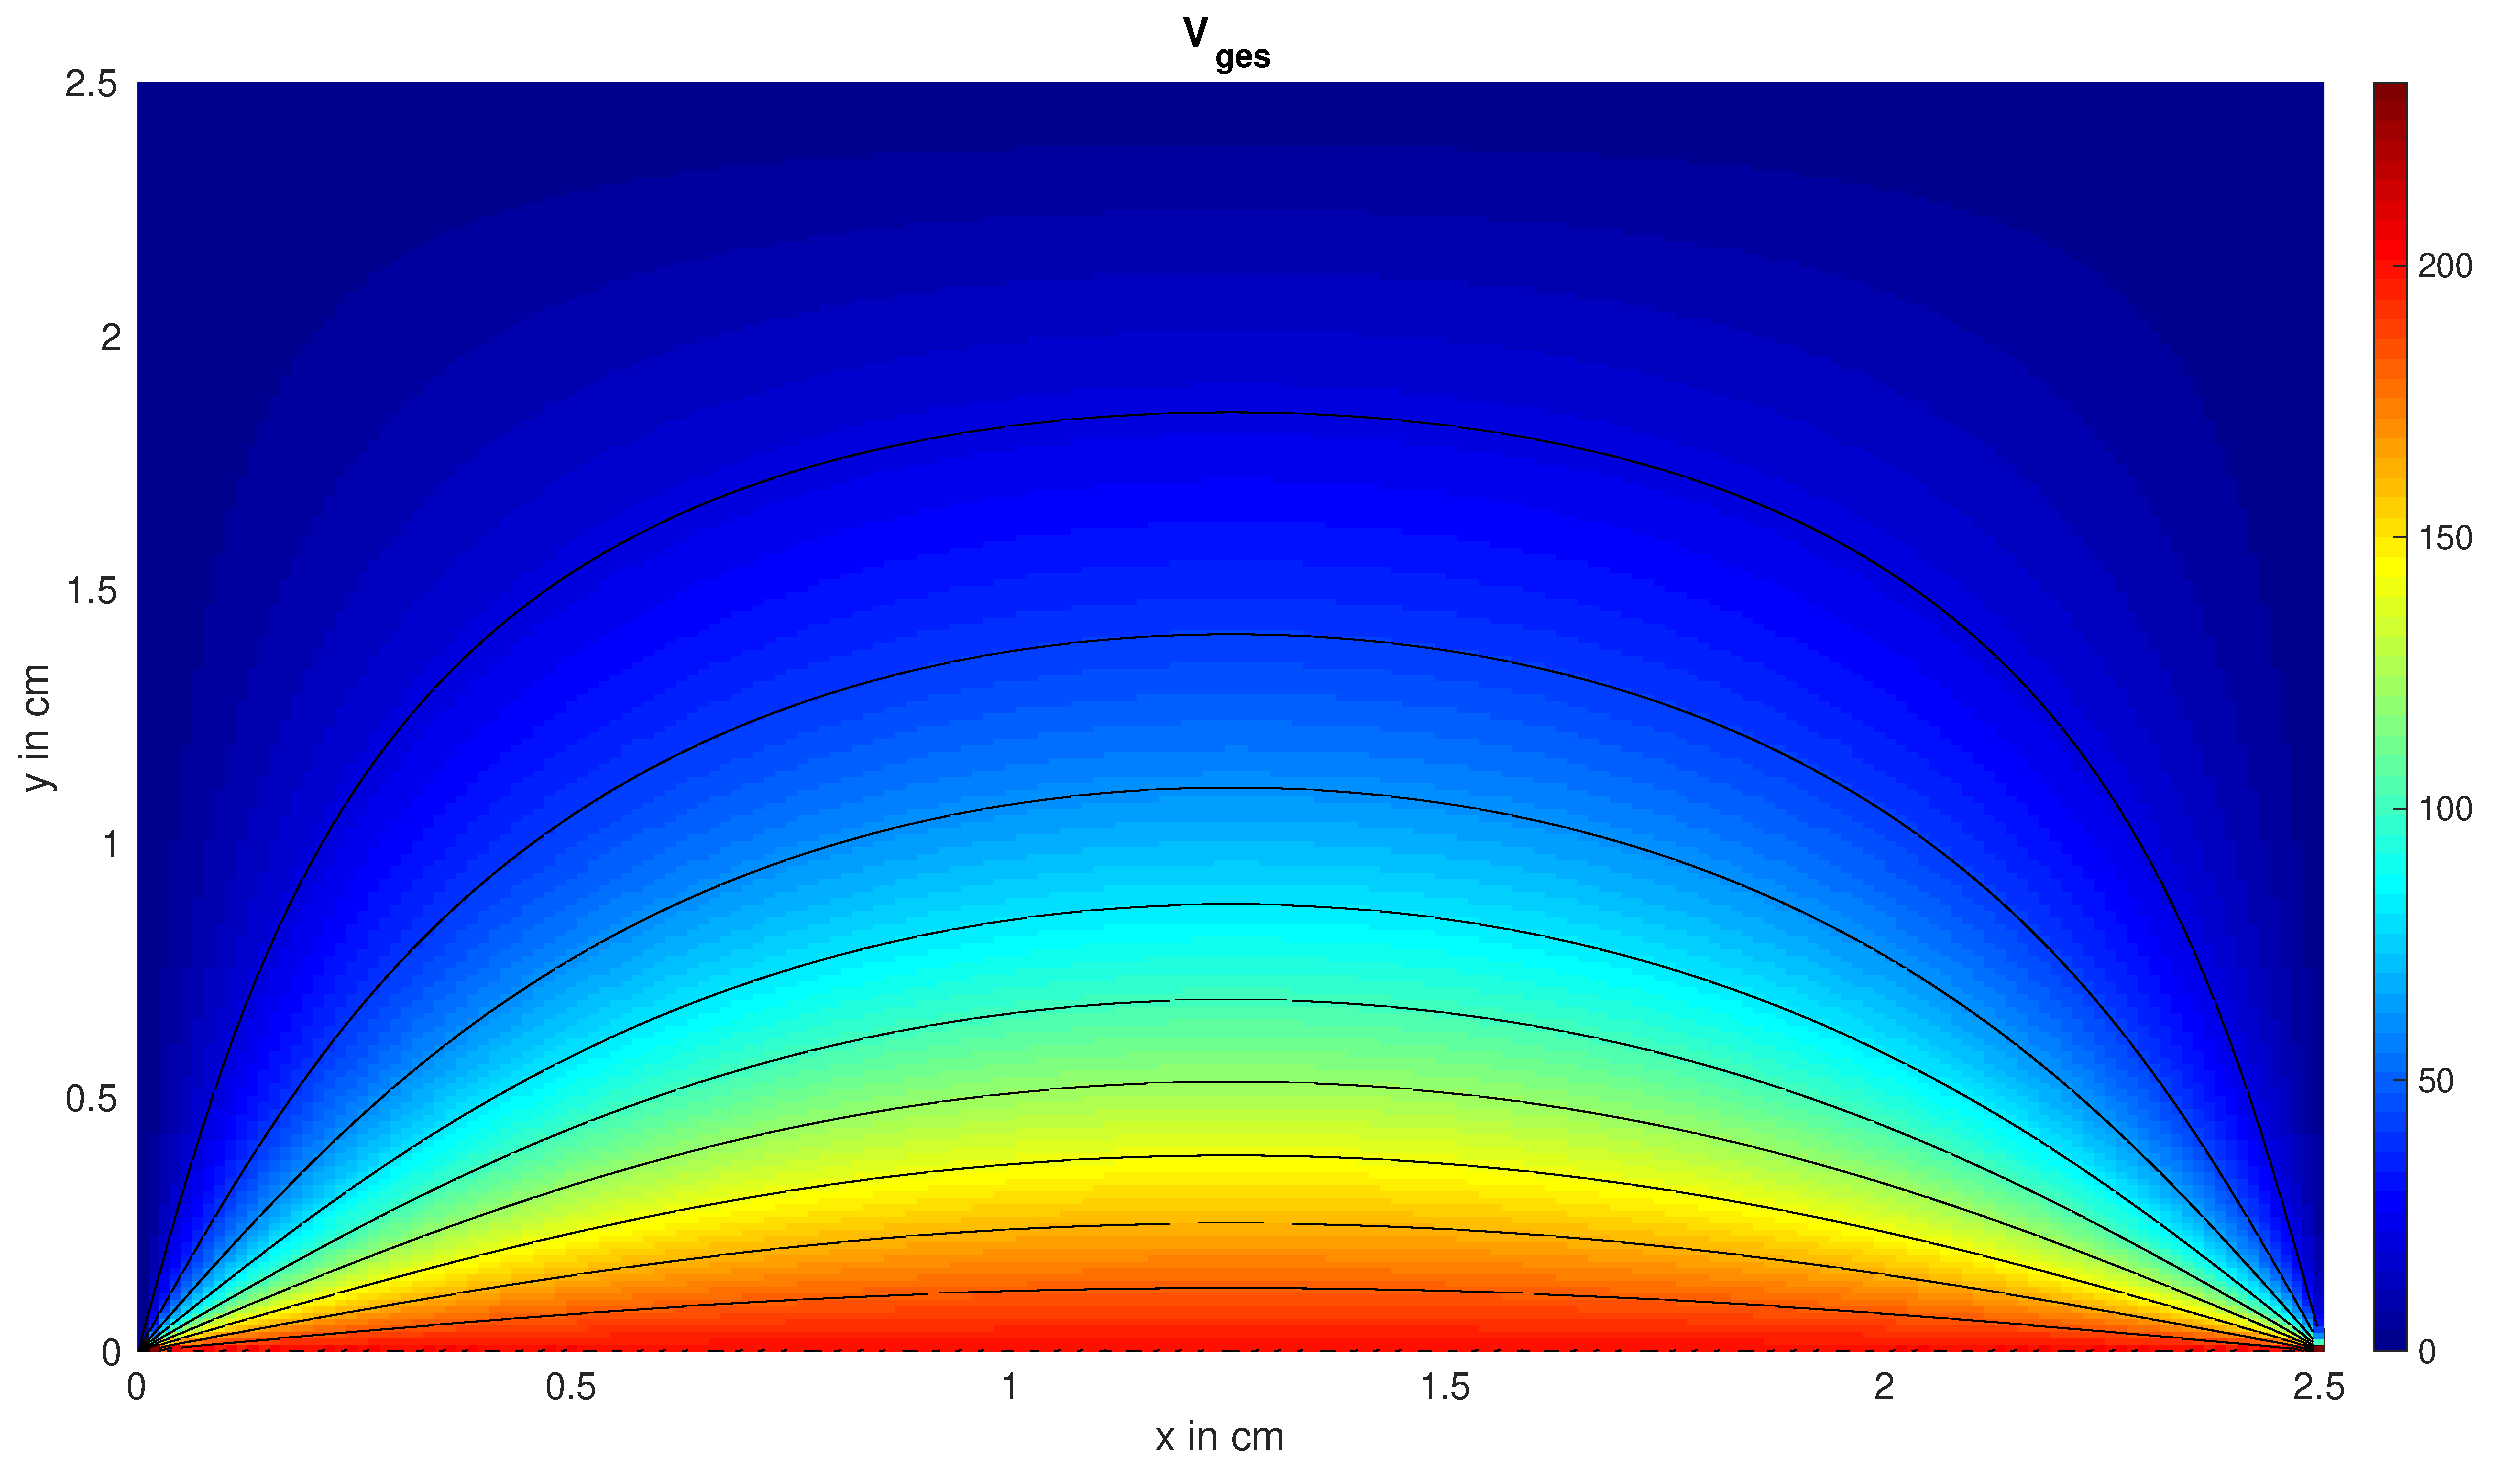
\includegraphics[width=1.0\textwidth]{pics/Bsp_1_analytical_figures/TaskA_fig_4.eps}
  \label{fig:Ana:TaskA:CompleteRot}
  \caption{Potentialverteilung der Gesamtlösung - Draufsicht}
\end{figure}

\newsubsubsection{Feldbild}{}
\begin{figure}[H]
  \centering
  		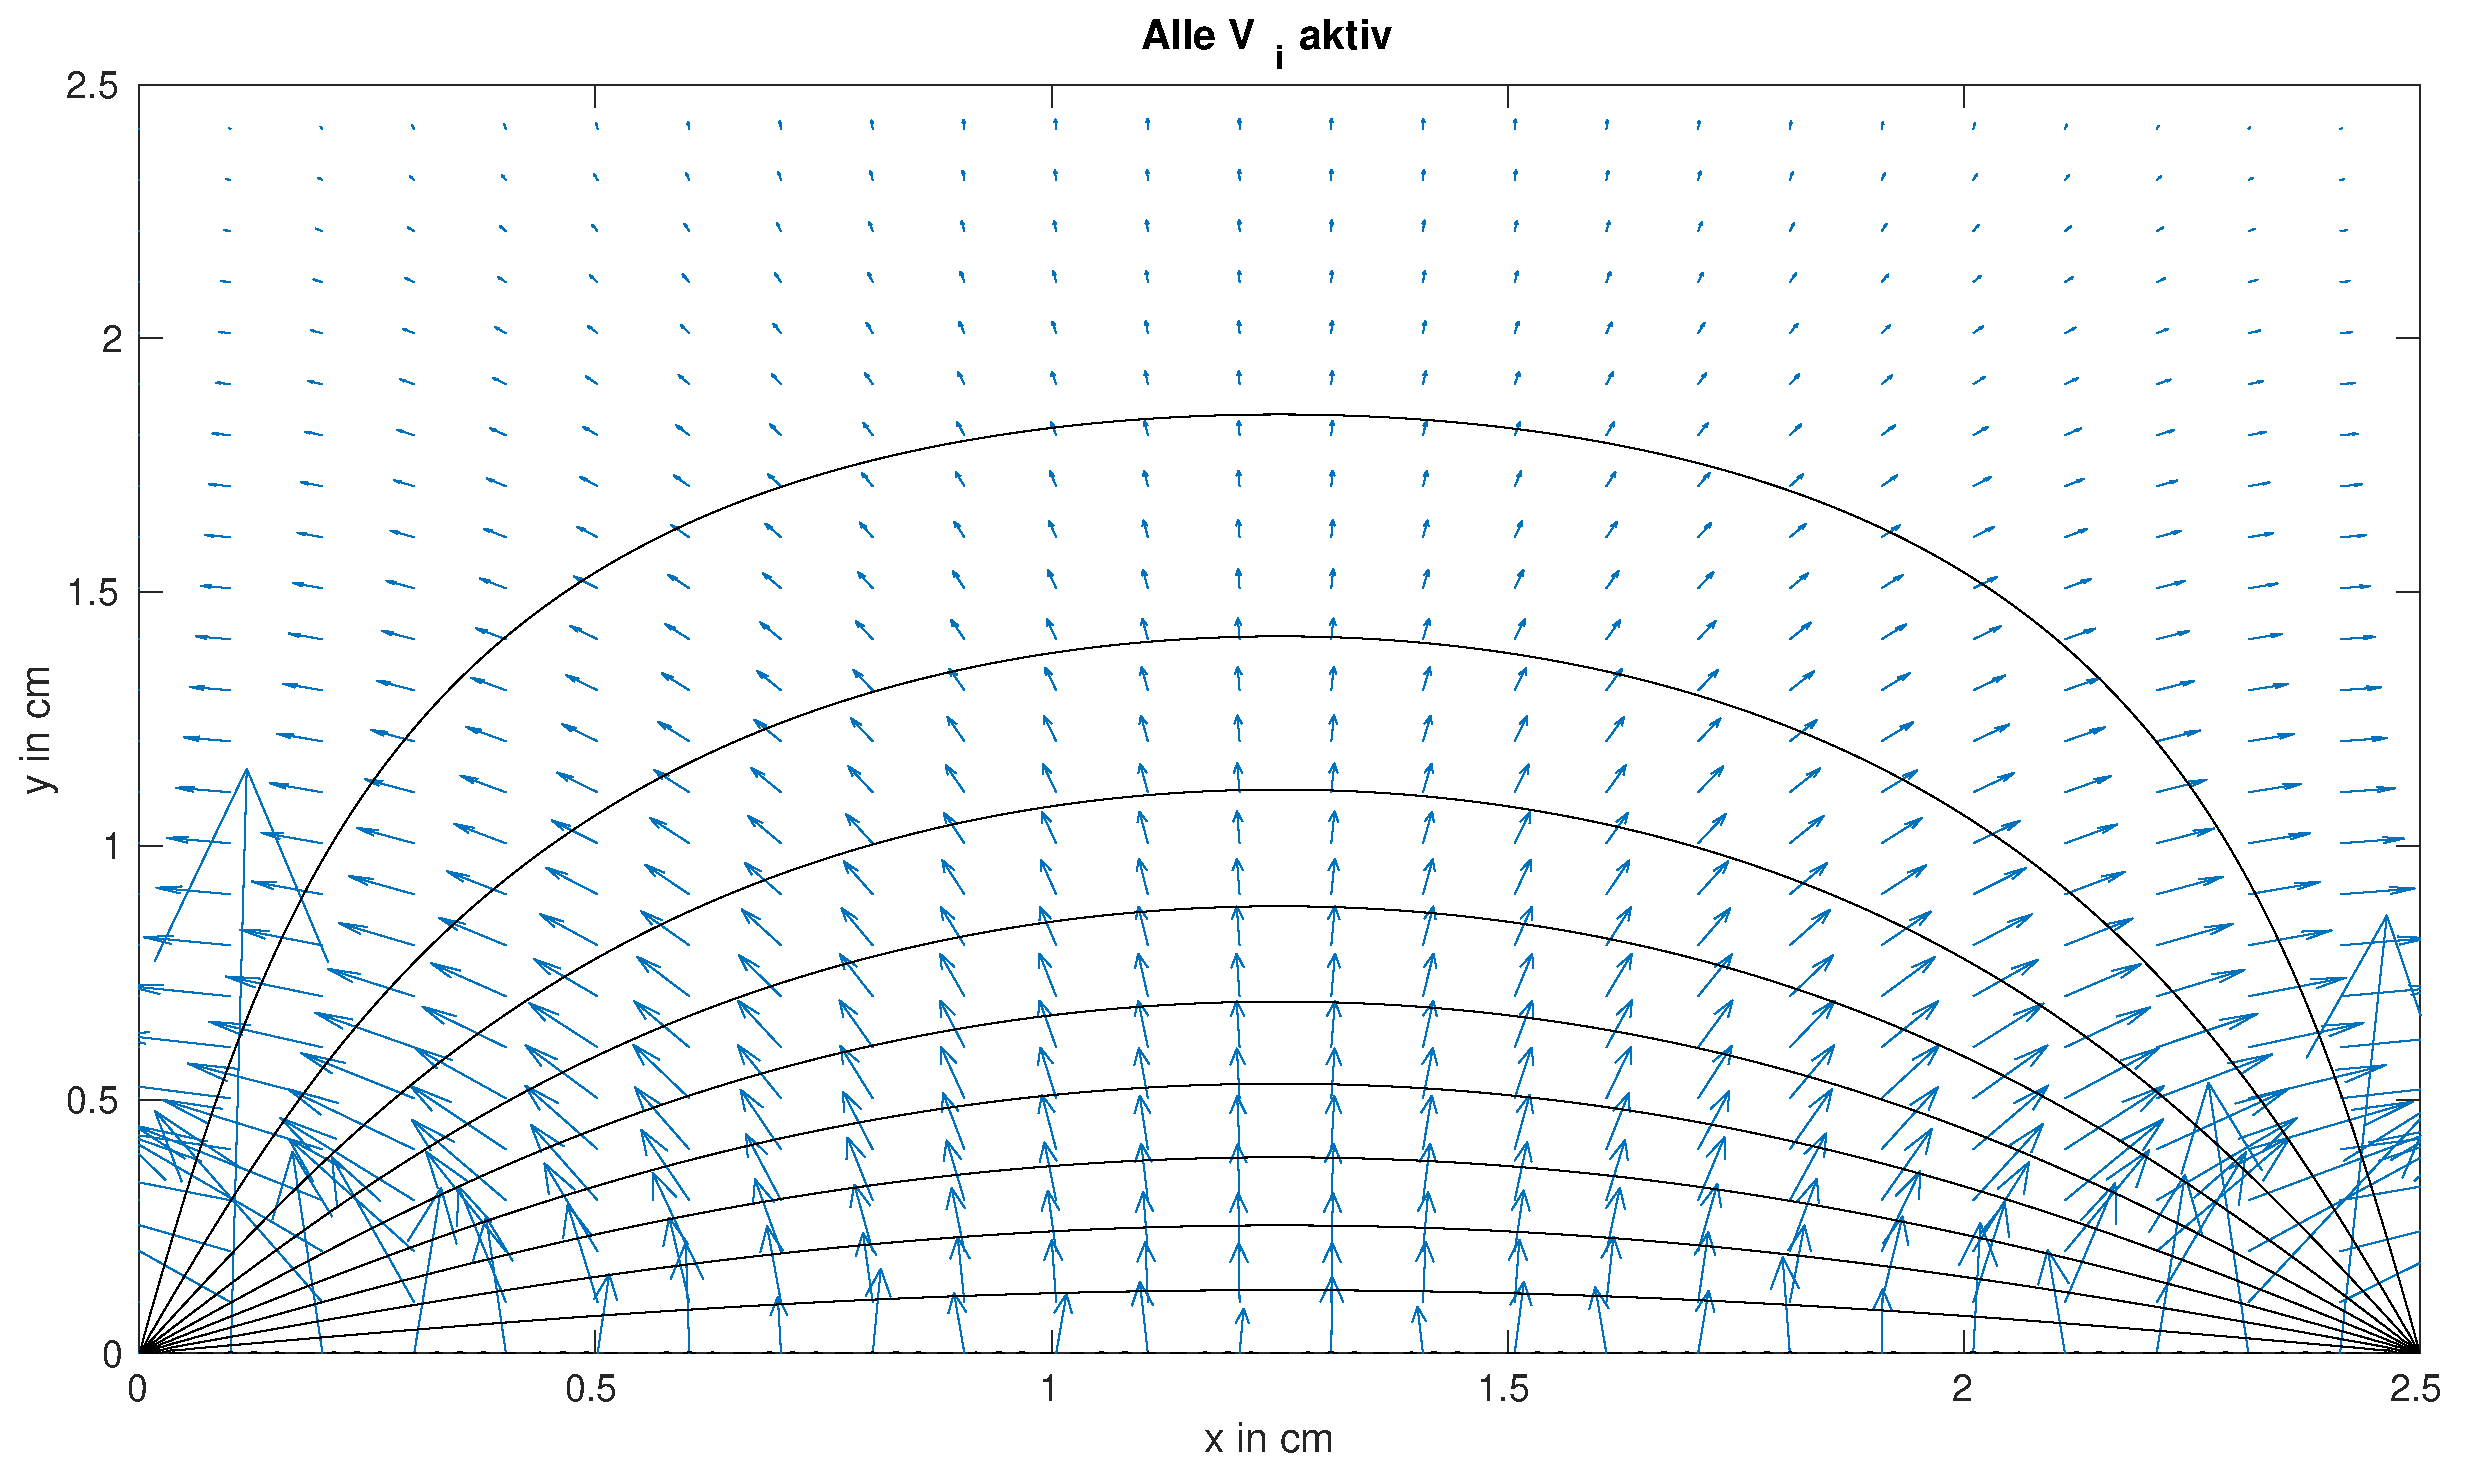
\includegraphics[width=1.0\textwidth]{pics/Bsp_1_analytical_figures/TaskA_fig_6.eps}
  \label{fig:Ana:TaskA:Field:Complete}
  \caption{Feldbild der Gesamtlösung mit Äquipotentiallinien}
\end{figure}


\newsubsection{Fall II}{}
Hier gilt für die einzelnen Potentiale der Metallplatten:
\begin{align*}
	&V_A = 500\,\mathrm{V} \\
	&V_B = 100\,\mathrm{V} \\
	&V_C = 0\,\mathrm{V} \\
	&V_D = 0\,\mathrm{V}
\end{align*}

\newsubsubsection{Teillösungen}{}
\begin{figure}[H]
  \centering
  		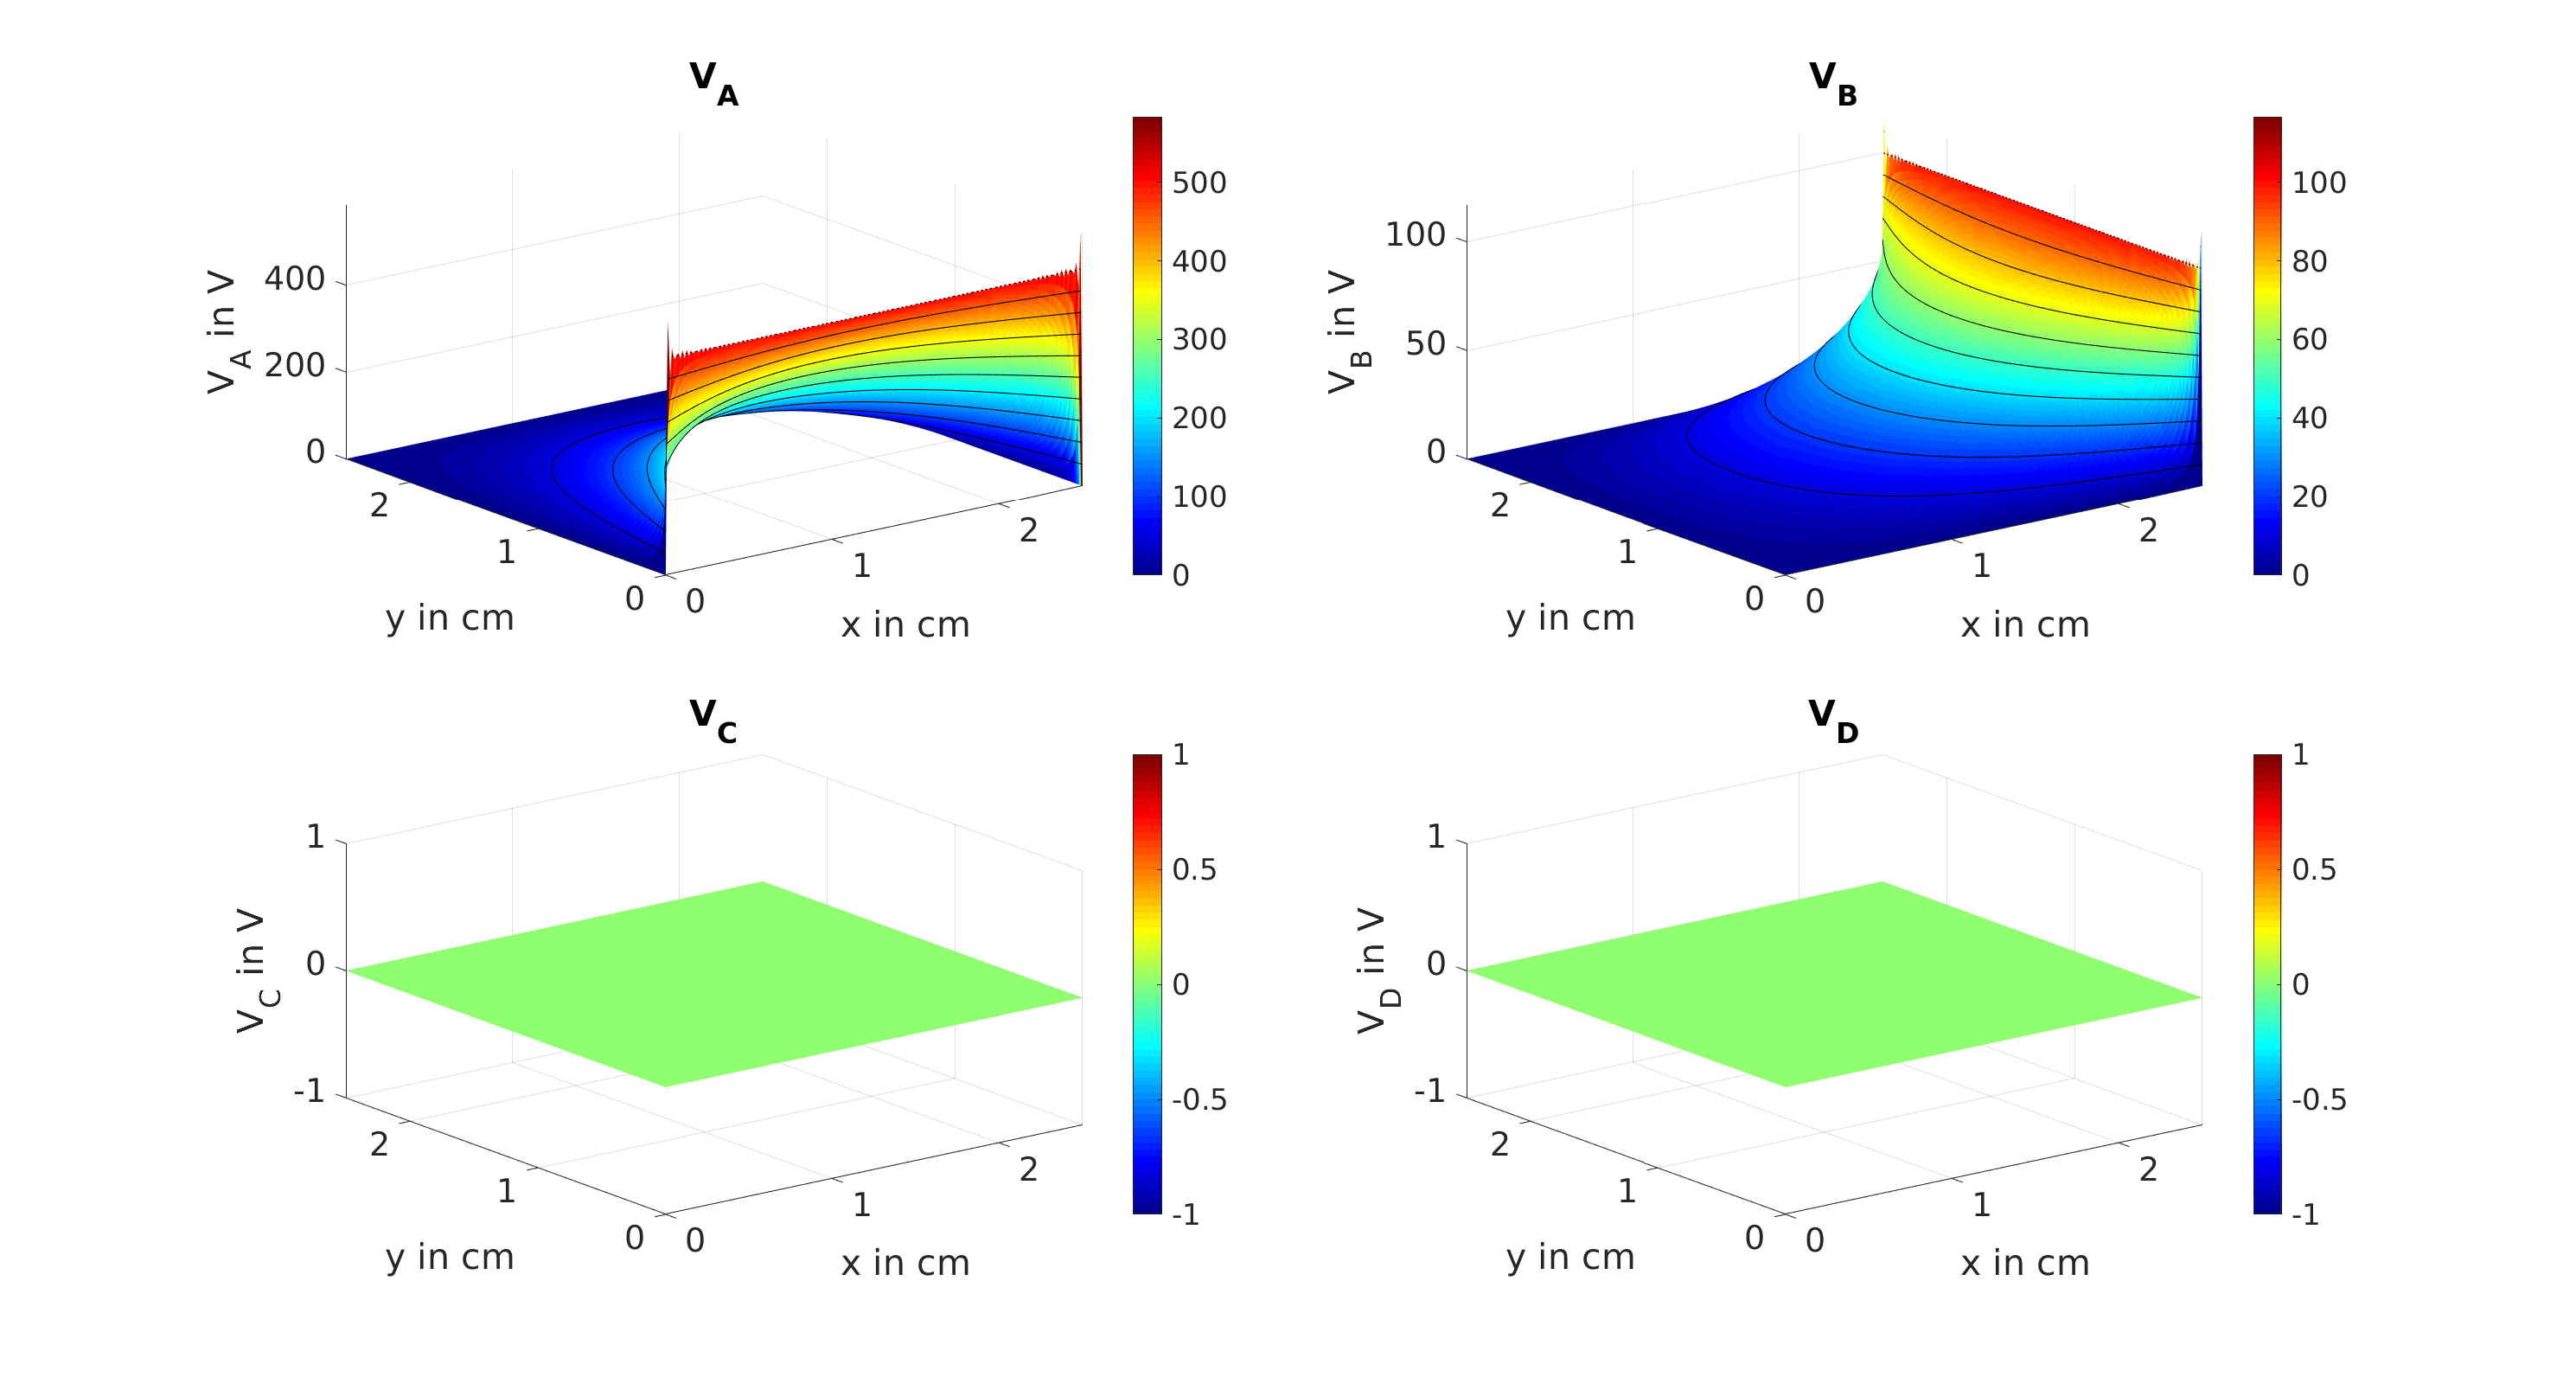
\includegraphics[width=1.0\textwidth]{pics/Bsp_1_analytical_figures/TaskB_fig_1.eps}
  \label{fig:Ana:TaskB:Individual}
  \caption{Potentialverteilung der einzelnen Teillösungen}
\end{figure}

\begin{figure}[H]
  \centering
  		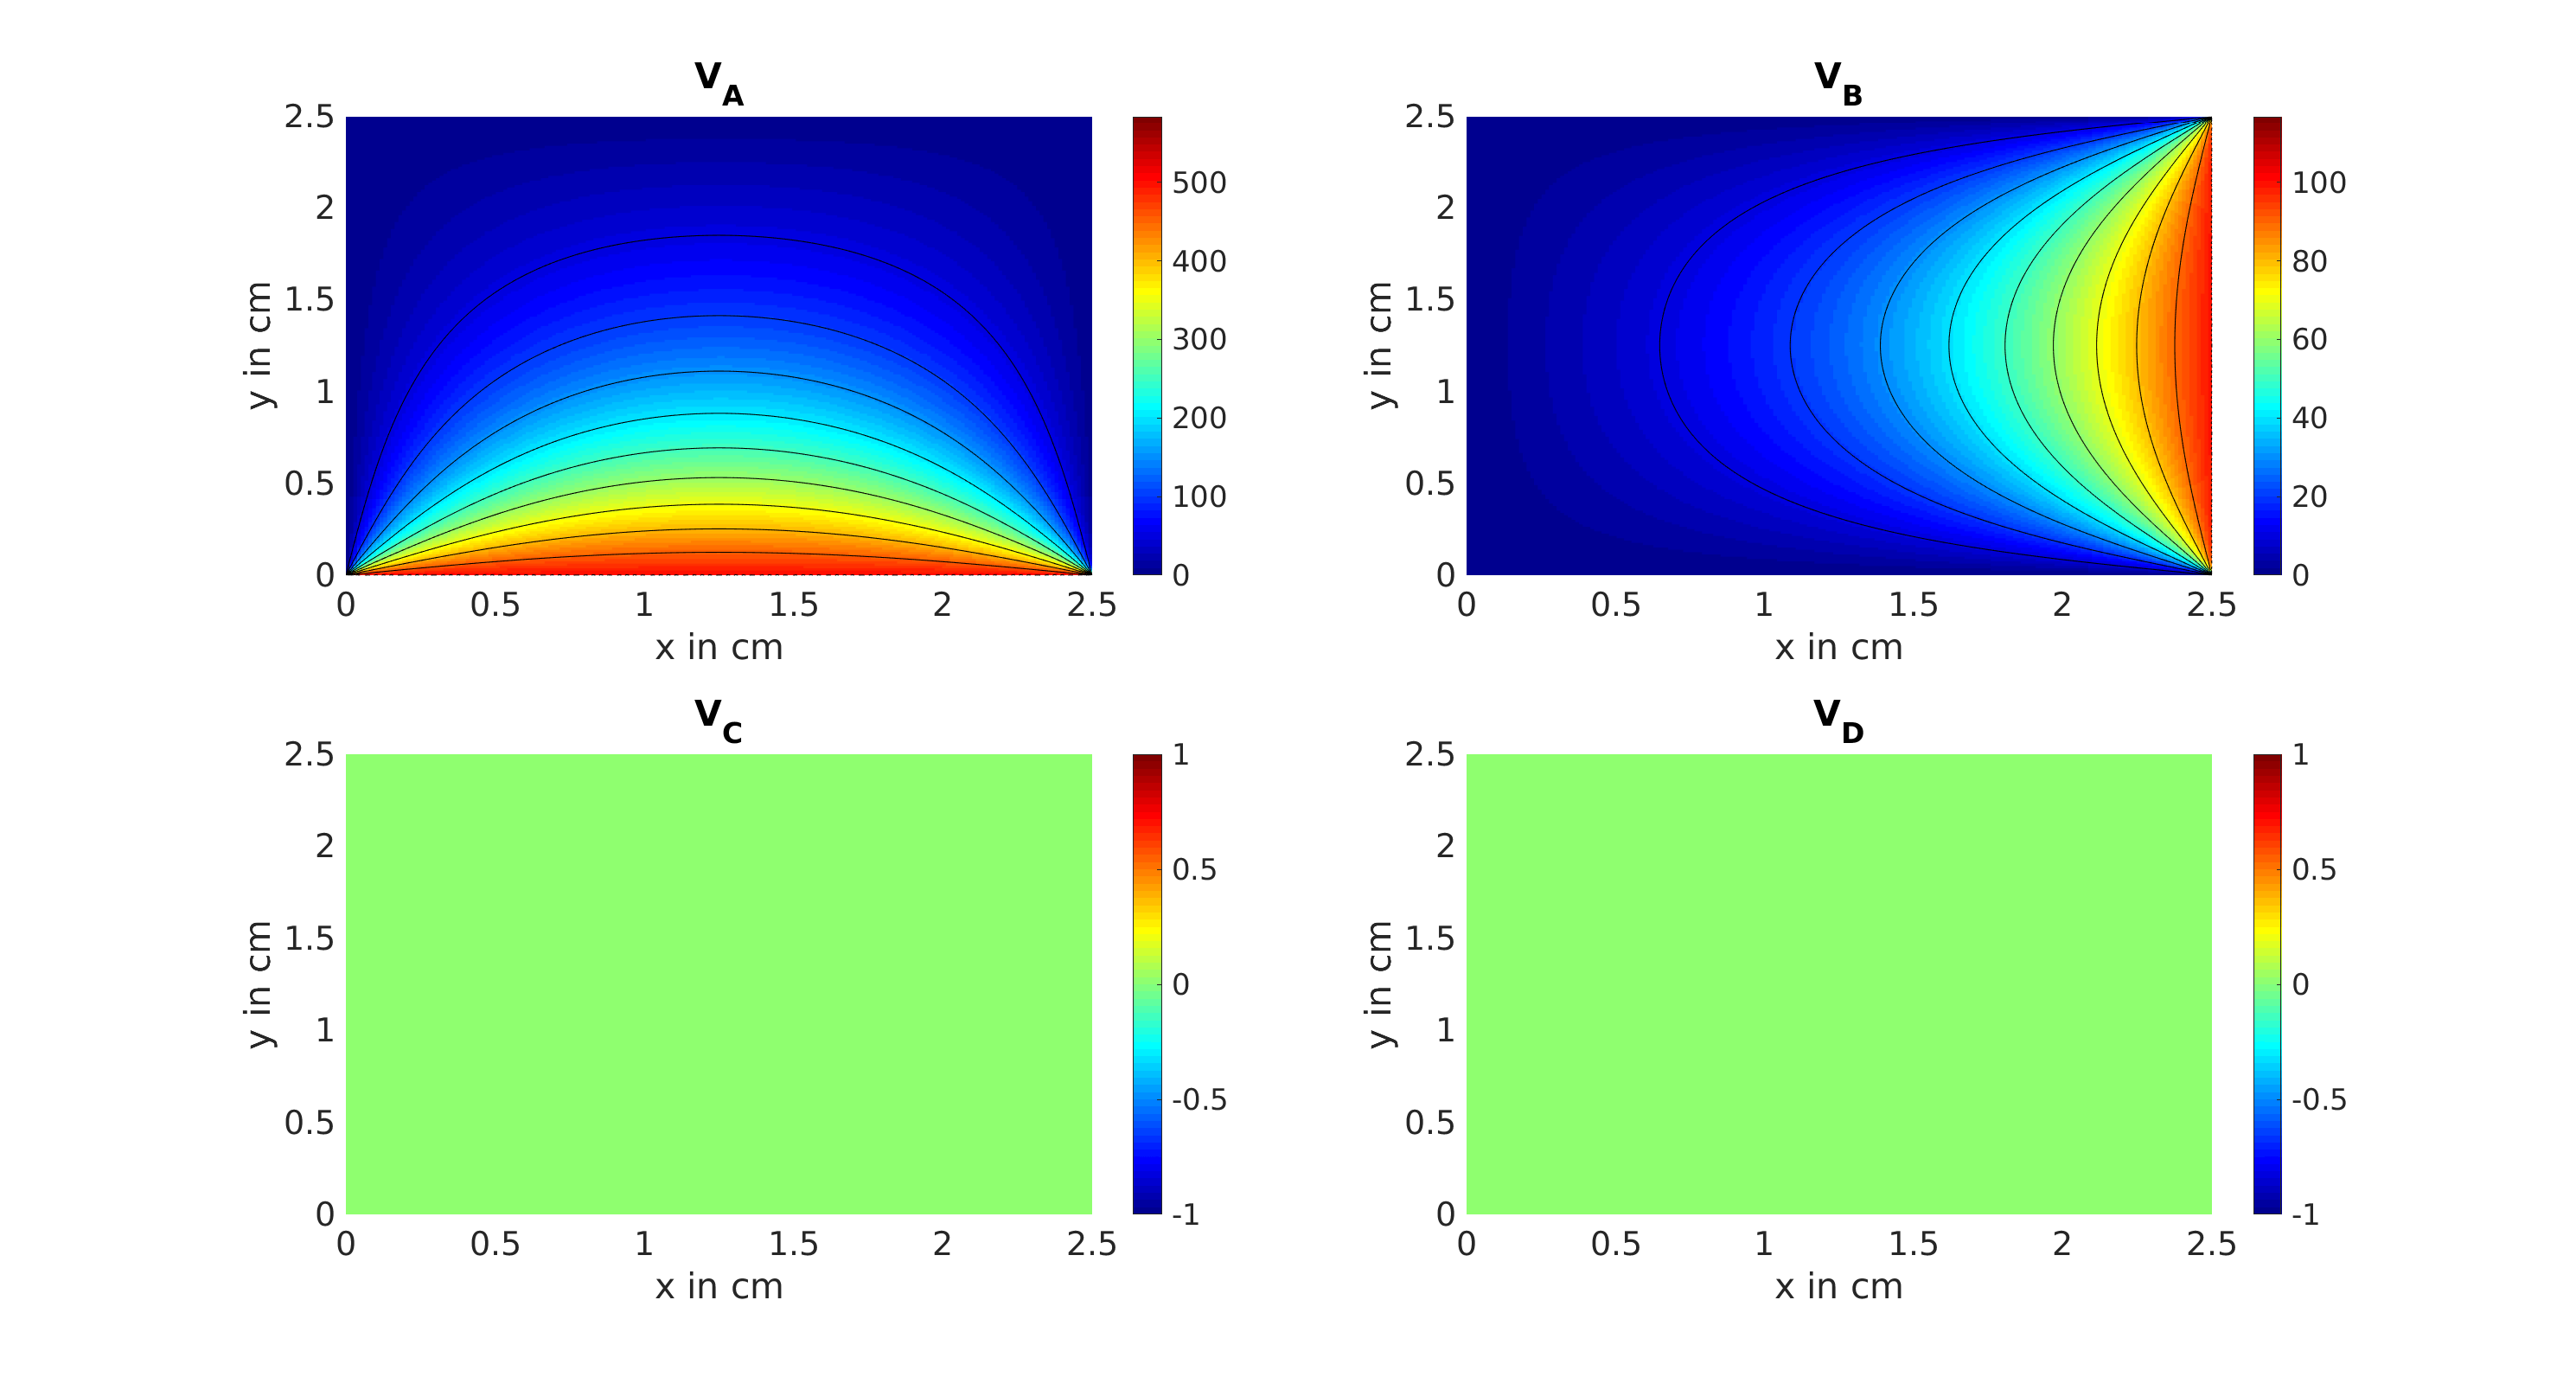
\includegraphics[width=1.0\textwidth]{pics/Bsp_1_analytical_figures/TaskB_fig_3.eps}
  \label{fig:Ana:TaskB:IndividualRot}
  \caption{Potentialverteilung der einzelnen Teillösungen - Draufsicht}
\end{figure}


\newsubsubsection{Gesamtlösung}{}
\begin{figure}[H]
  \centering
  		\includegraphics[width=1.0\textwidth]{pics/Bsp_1_analytical_figures/TaskB_fig_2.eps}
  \label{fig:Ana:TaskB:Complete}
  \caption{Potentialverteilung der Gesamtlösung}
\end{figure}

\begin{figure}[H]
  \centering
  		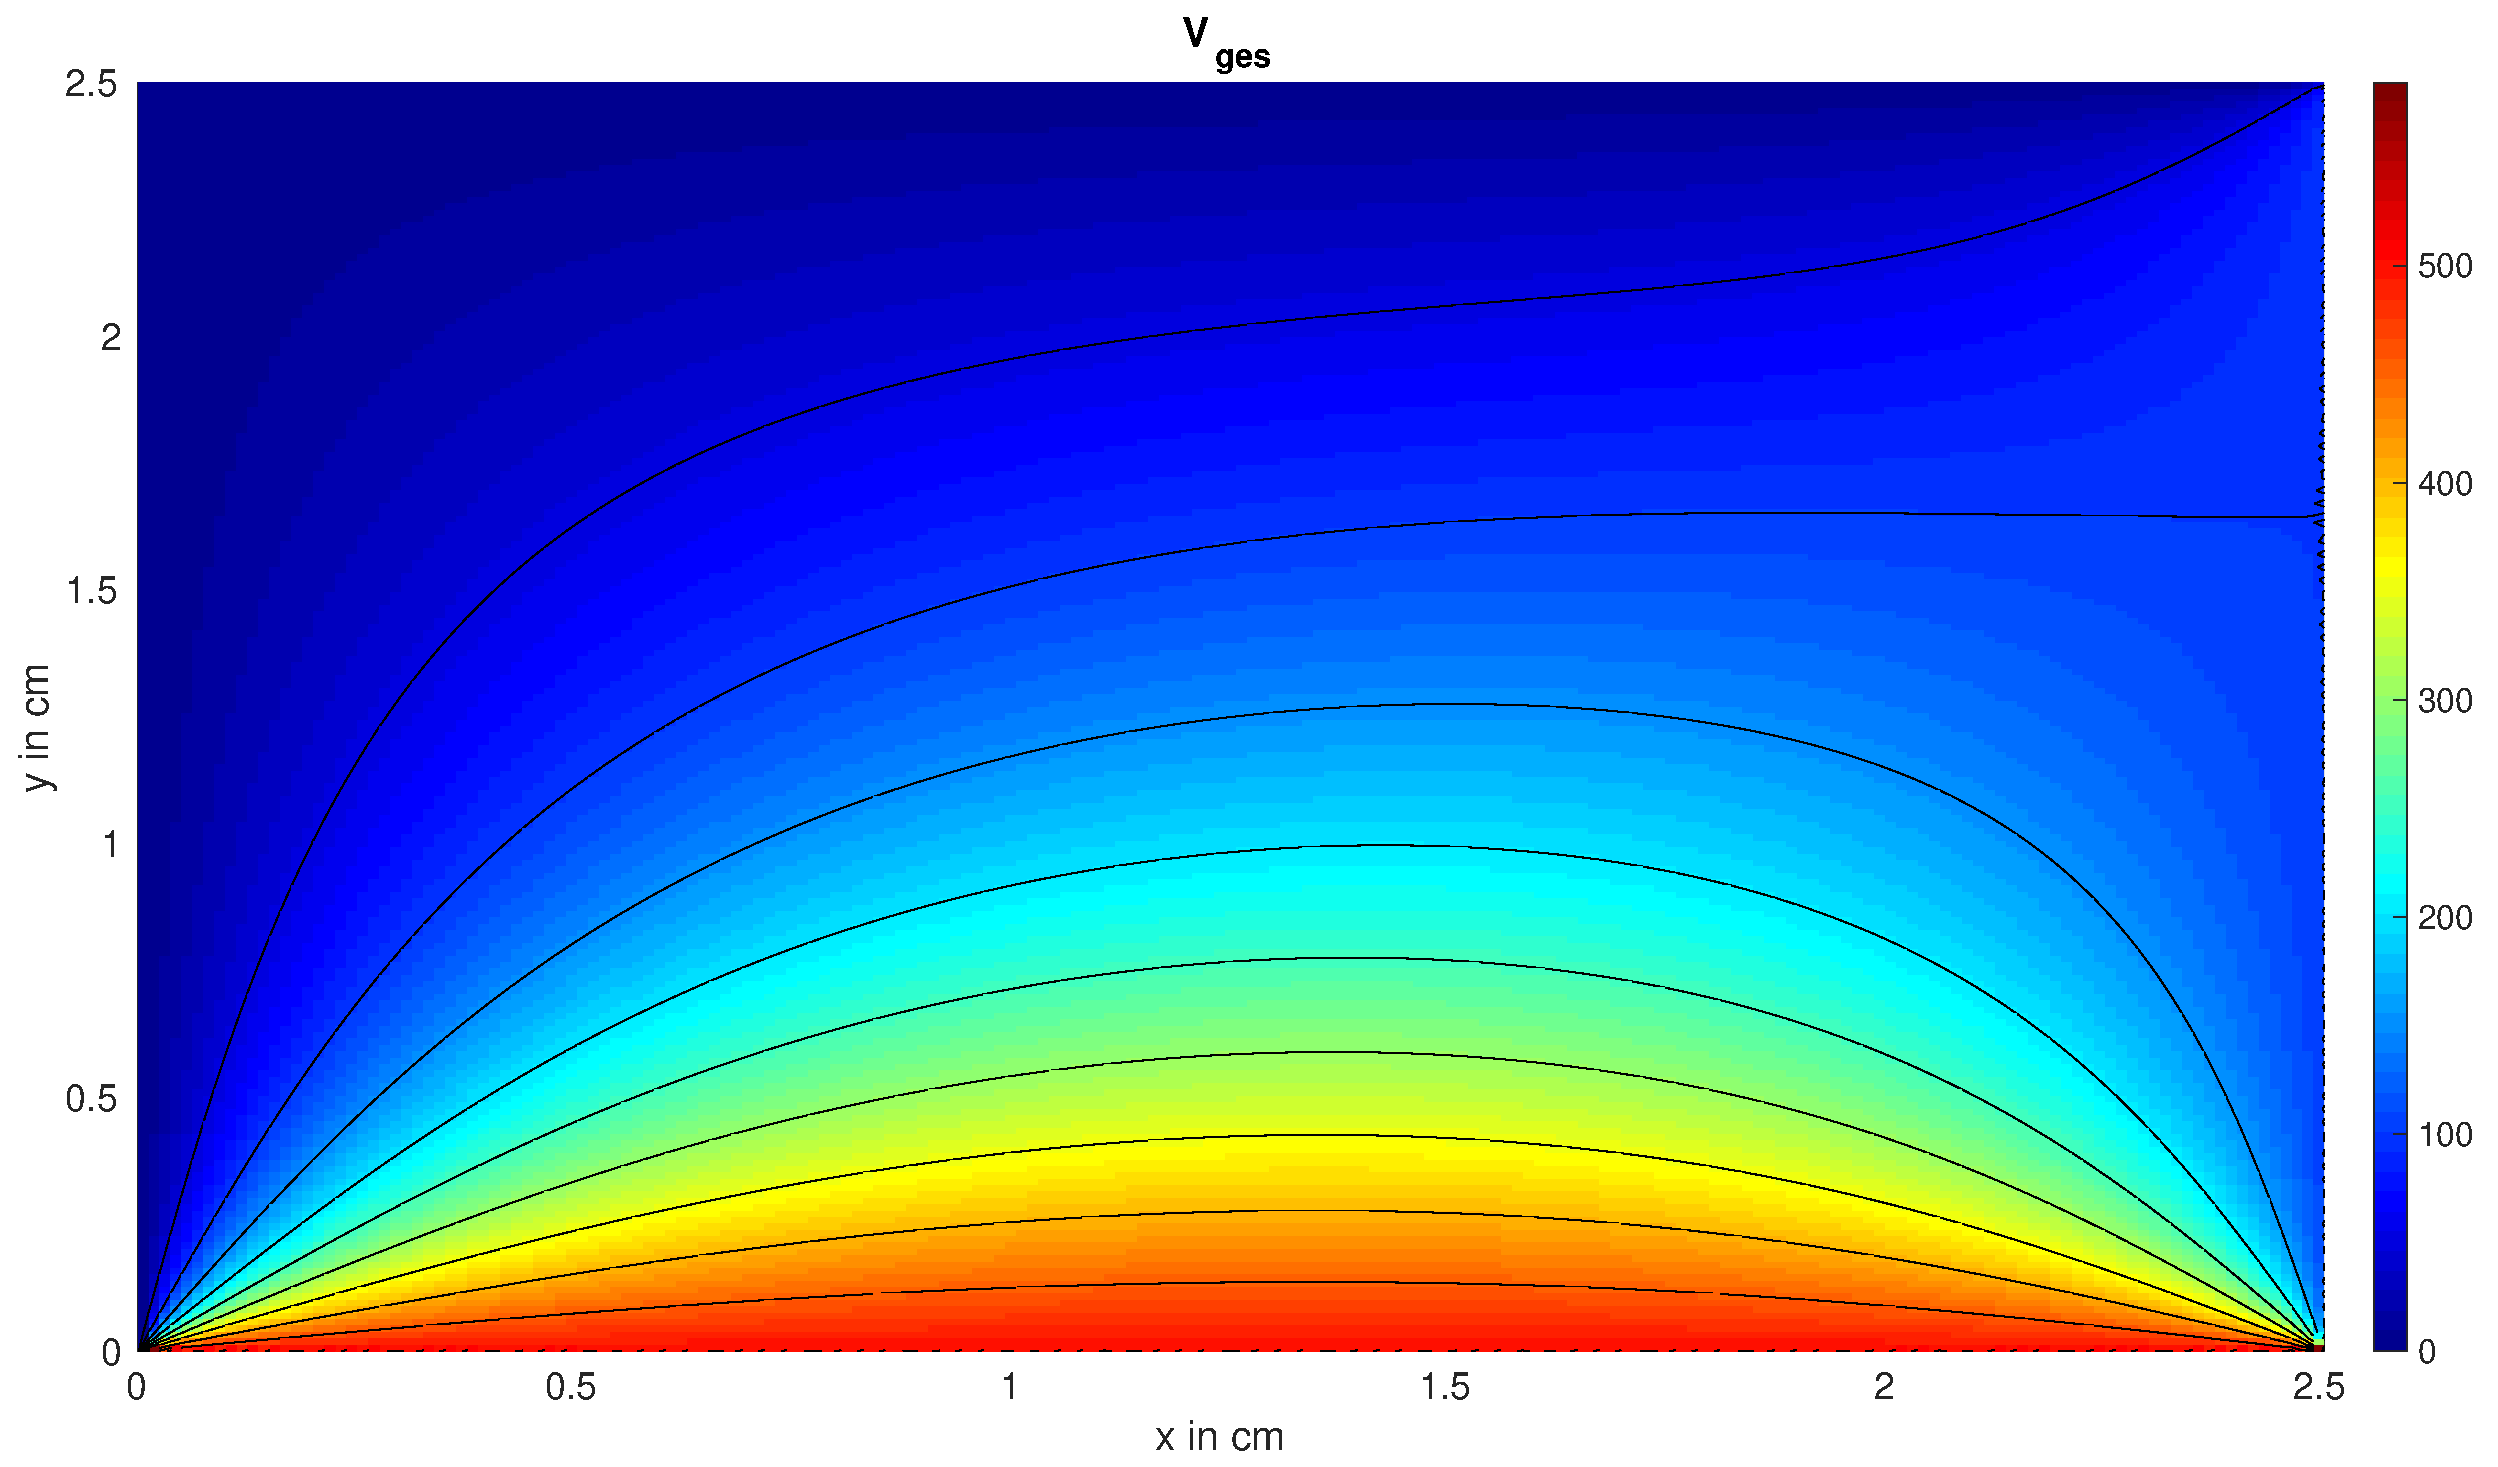
\includegraphics[width=1.0\textwidth]{pics/Bsp_1_analytical_figures/TaskB_fig_4.eps}
  \label{fig:Ana:TaskB:CompleteRot}
  \caption{Potentialverteilung der Gesamtlösung - Draufsicht}
\end{figure}

\newsubsubsection{Feldbild}{}
\begin{figure}[H]
  \centering
  		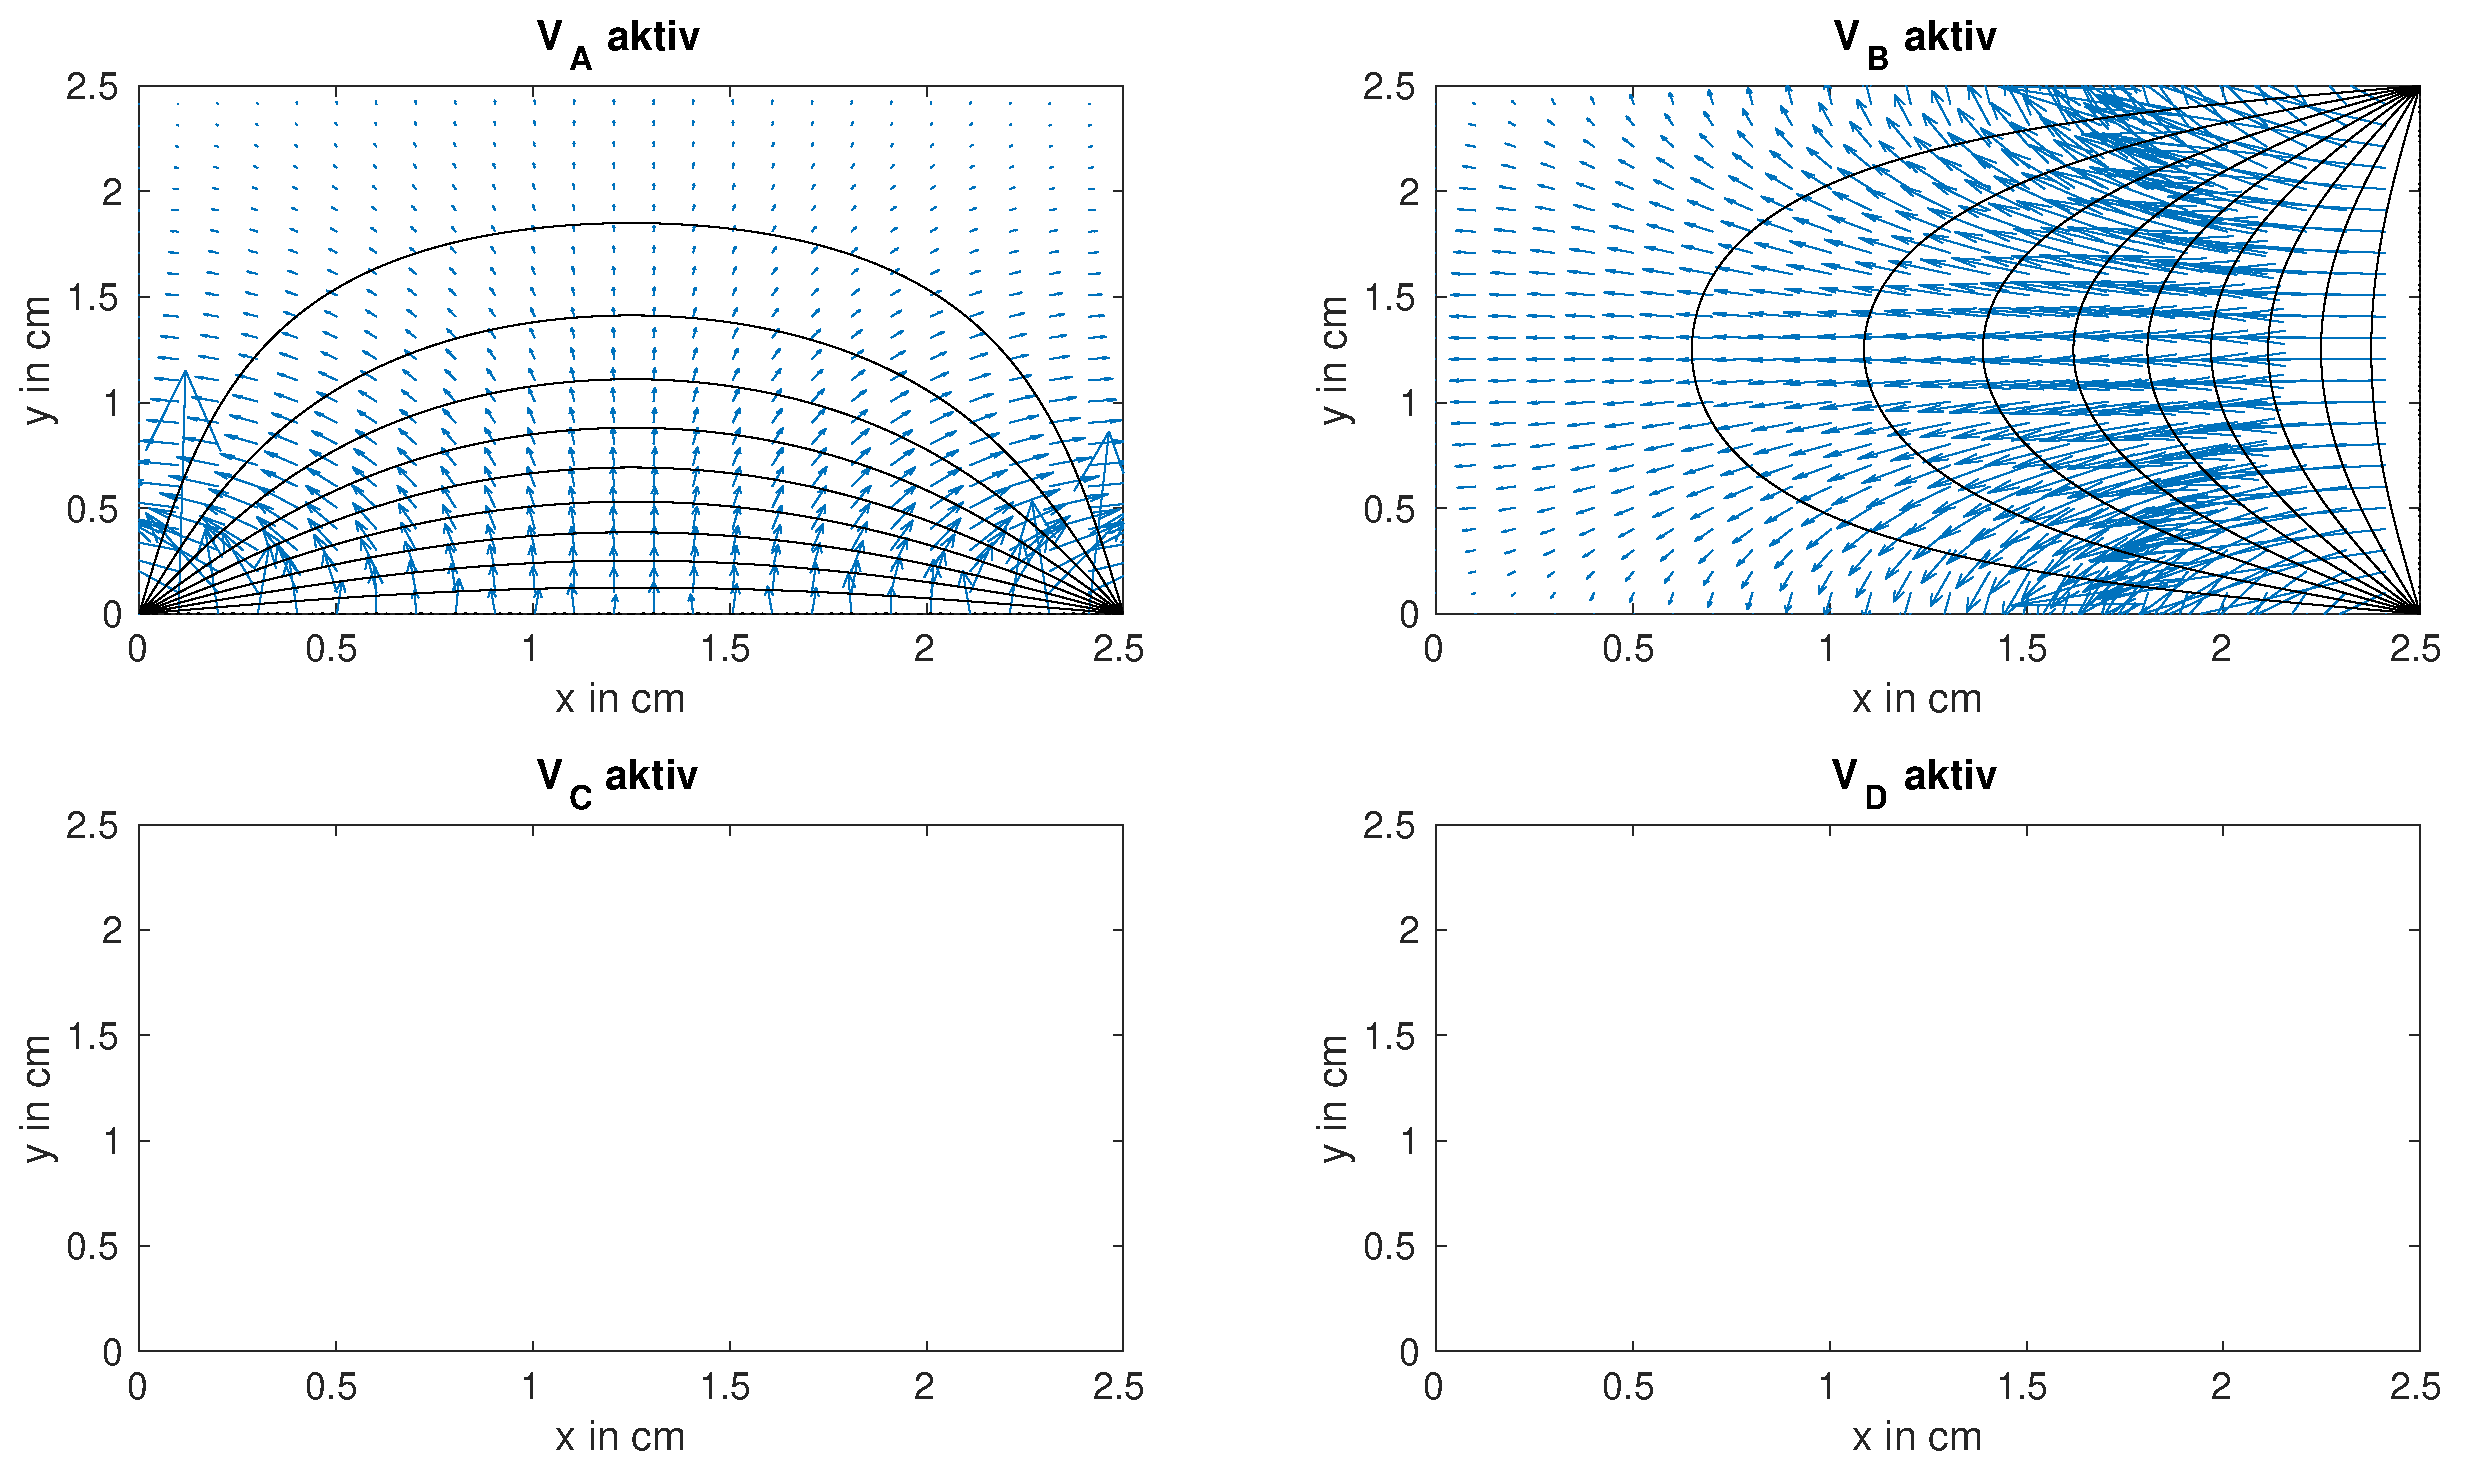
\includegraphics[width=1.0\textwidth]{pics/Bsp_1_analytical_figures/TaskB_fig_5.eps}
  \label{fig:Ana:TaskB:Field:Individual}
  \caption{Feldbild der einzelnen Teillösungen mit Äquipotentiallinien}
\end{figure}

\begin{figure}[H]
  \centering
  		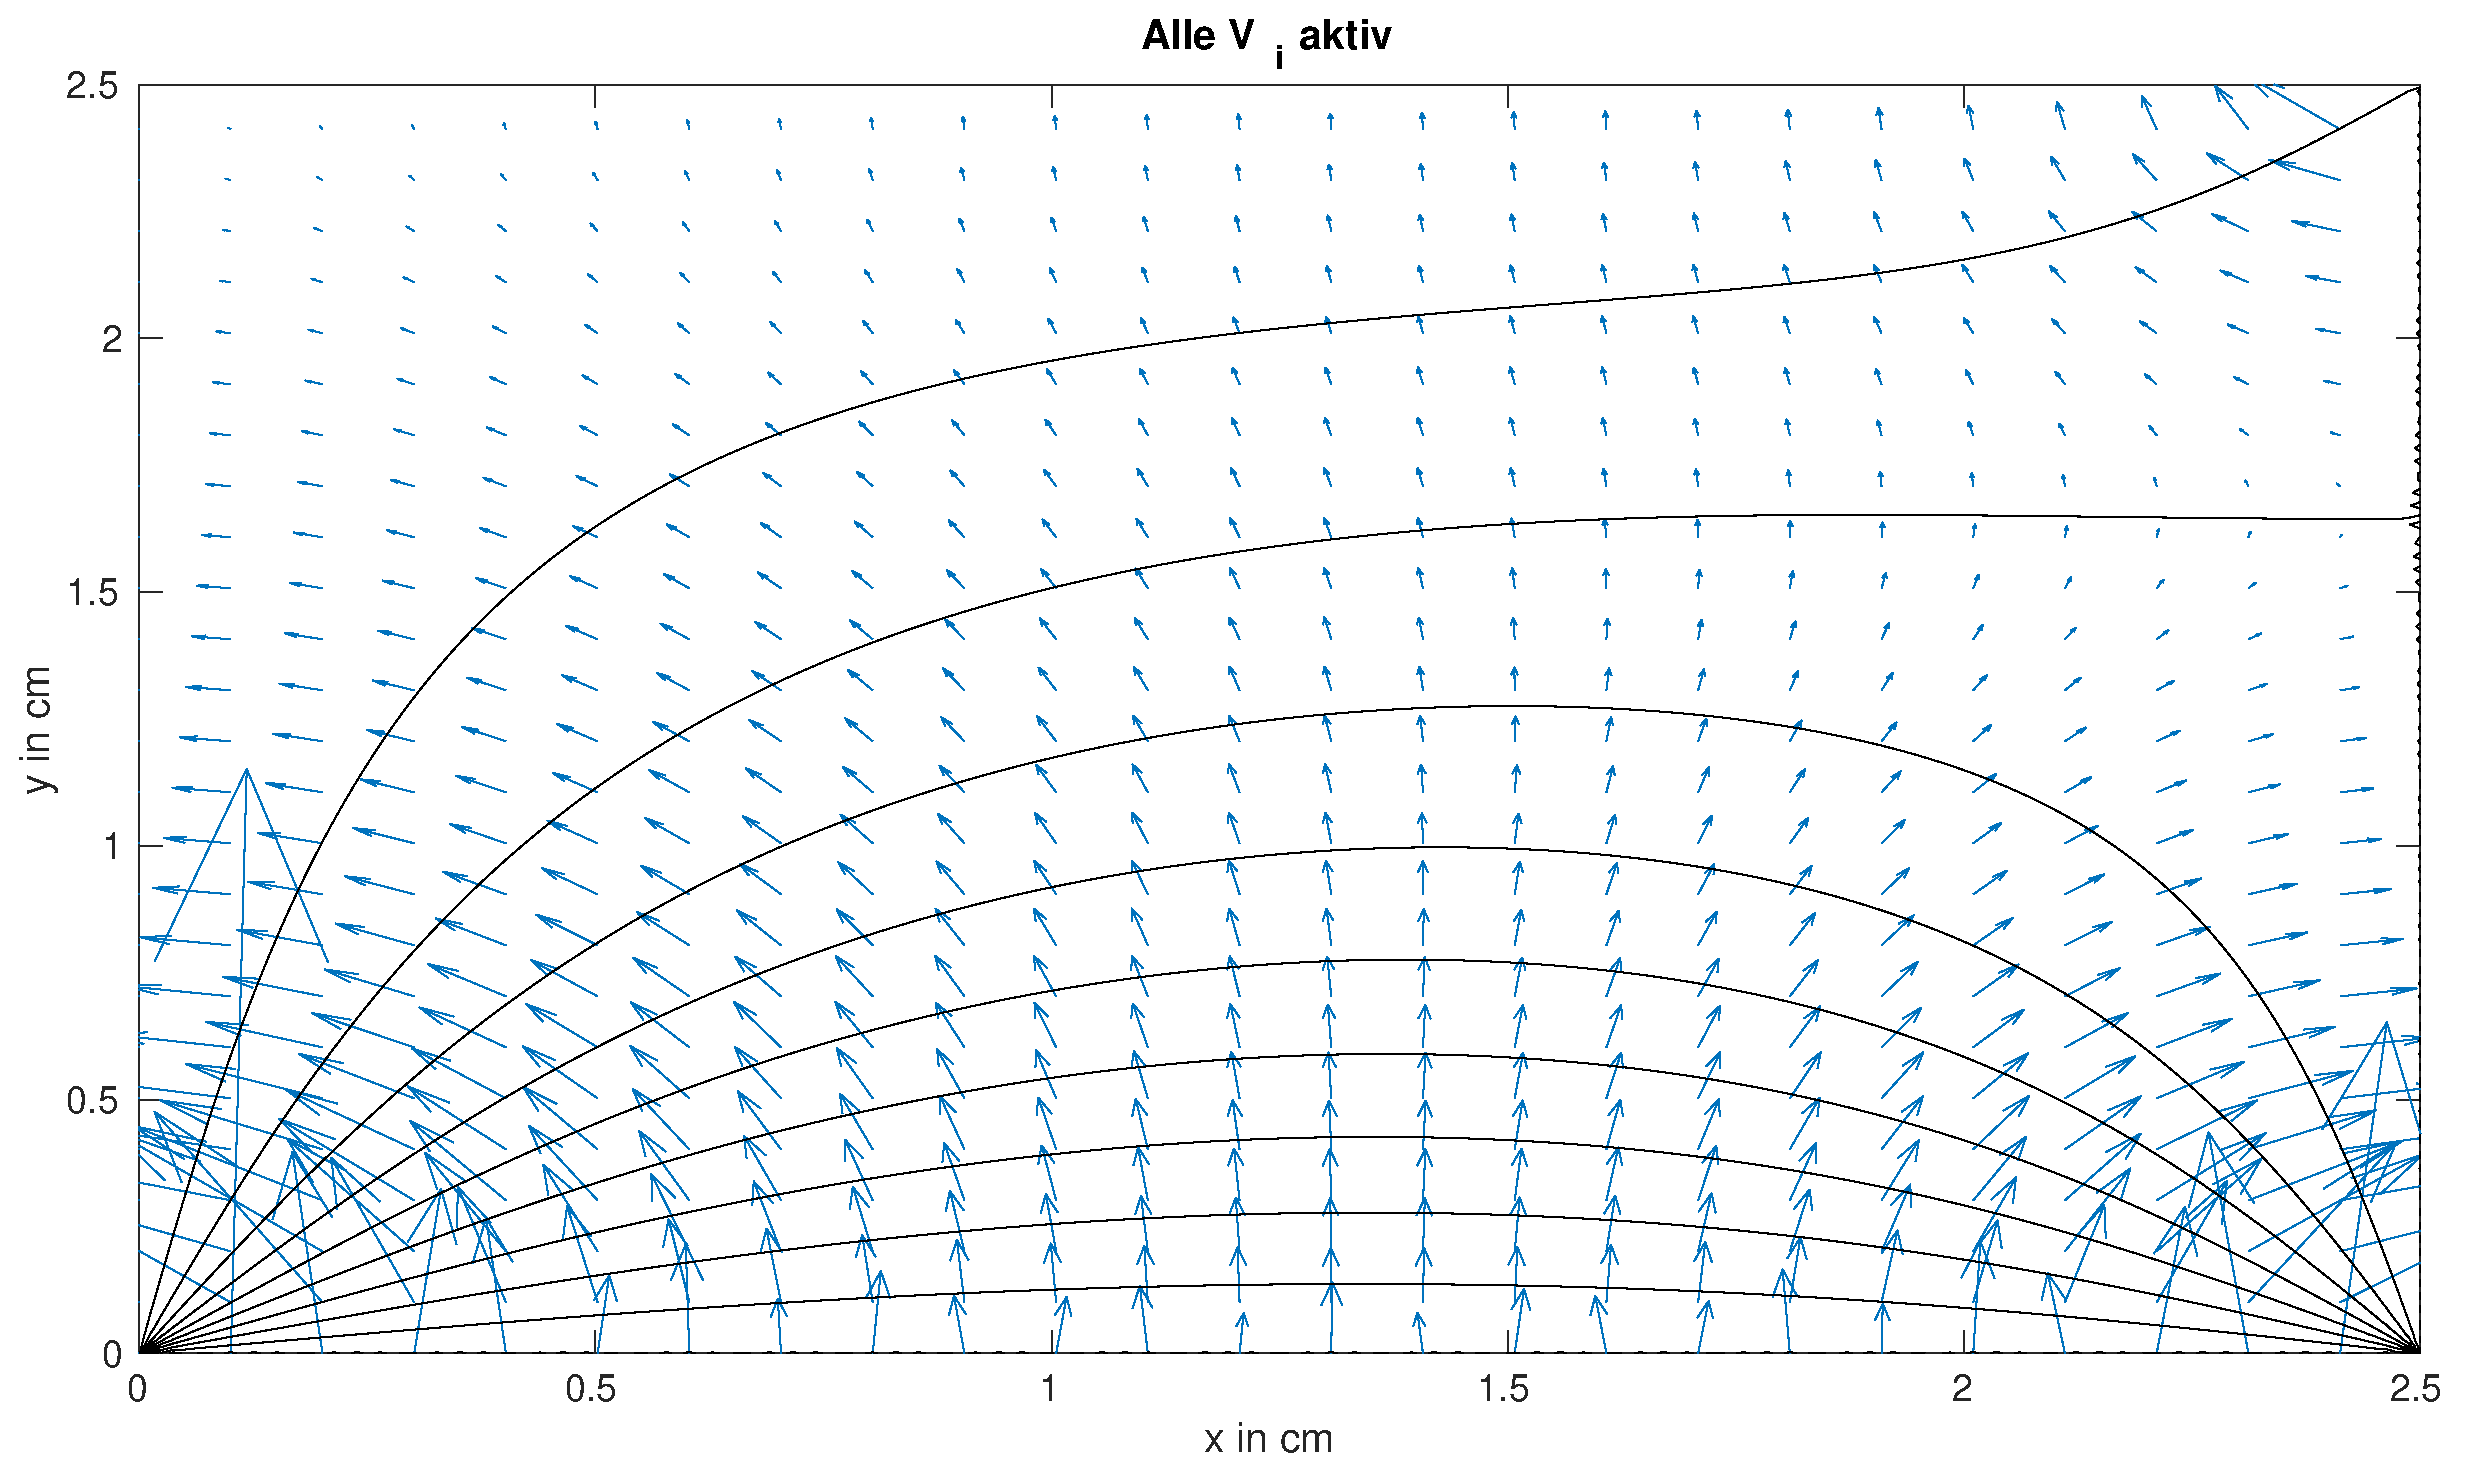
\includegraphics[width=1.0\textwidth]{pics/Bsp_1_analytical_figures/TaskB_fig_6.eps}
  \label{fig:Ana:TaskB:Field:Complete}
  \caption{Feldbild der Gesamtlösung mit Äquipotentiallinien}
\end{figure}



\newsubsection{Fall III}{}
Hier gilt für die einzelnen Potentiale der Metallplatten:
\begin{align*}
	&V_A = 500\,\mathrm{V} \\
	&V_B = 100\,\mathrm{V} \\
	&V_C = 300\,\mathrm{V} \\
	&V_D = 400\,\mathrm{V}
\end{align*}

\newsubsubsection{Teillösungen}{}
\begin{figure}[H]
  \centering
  		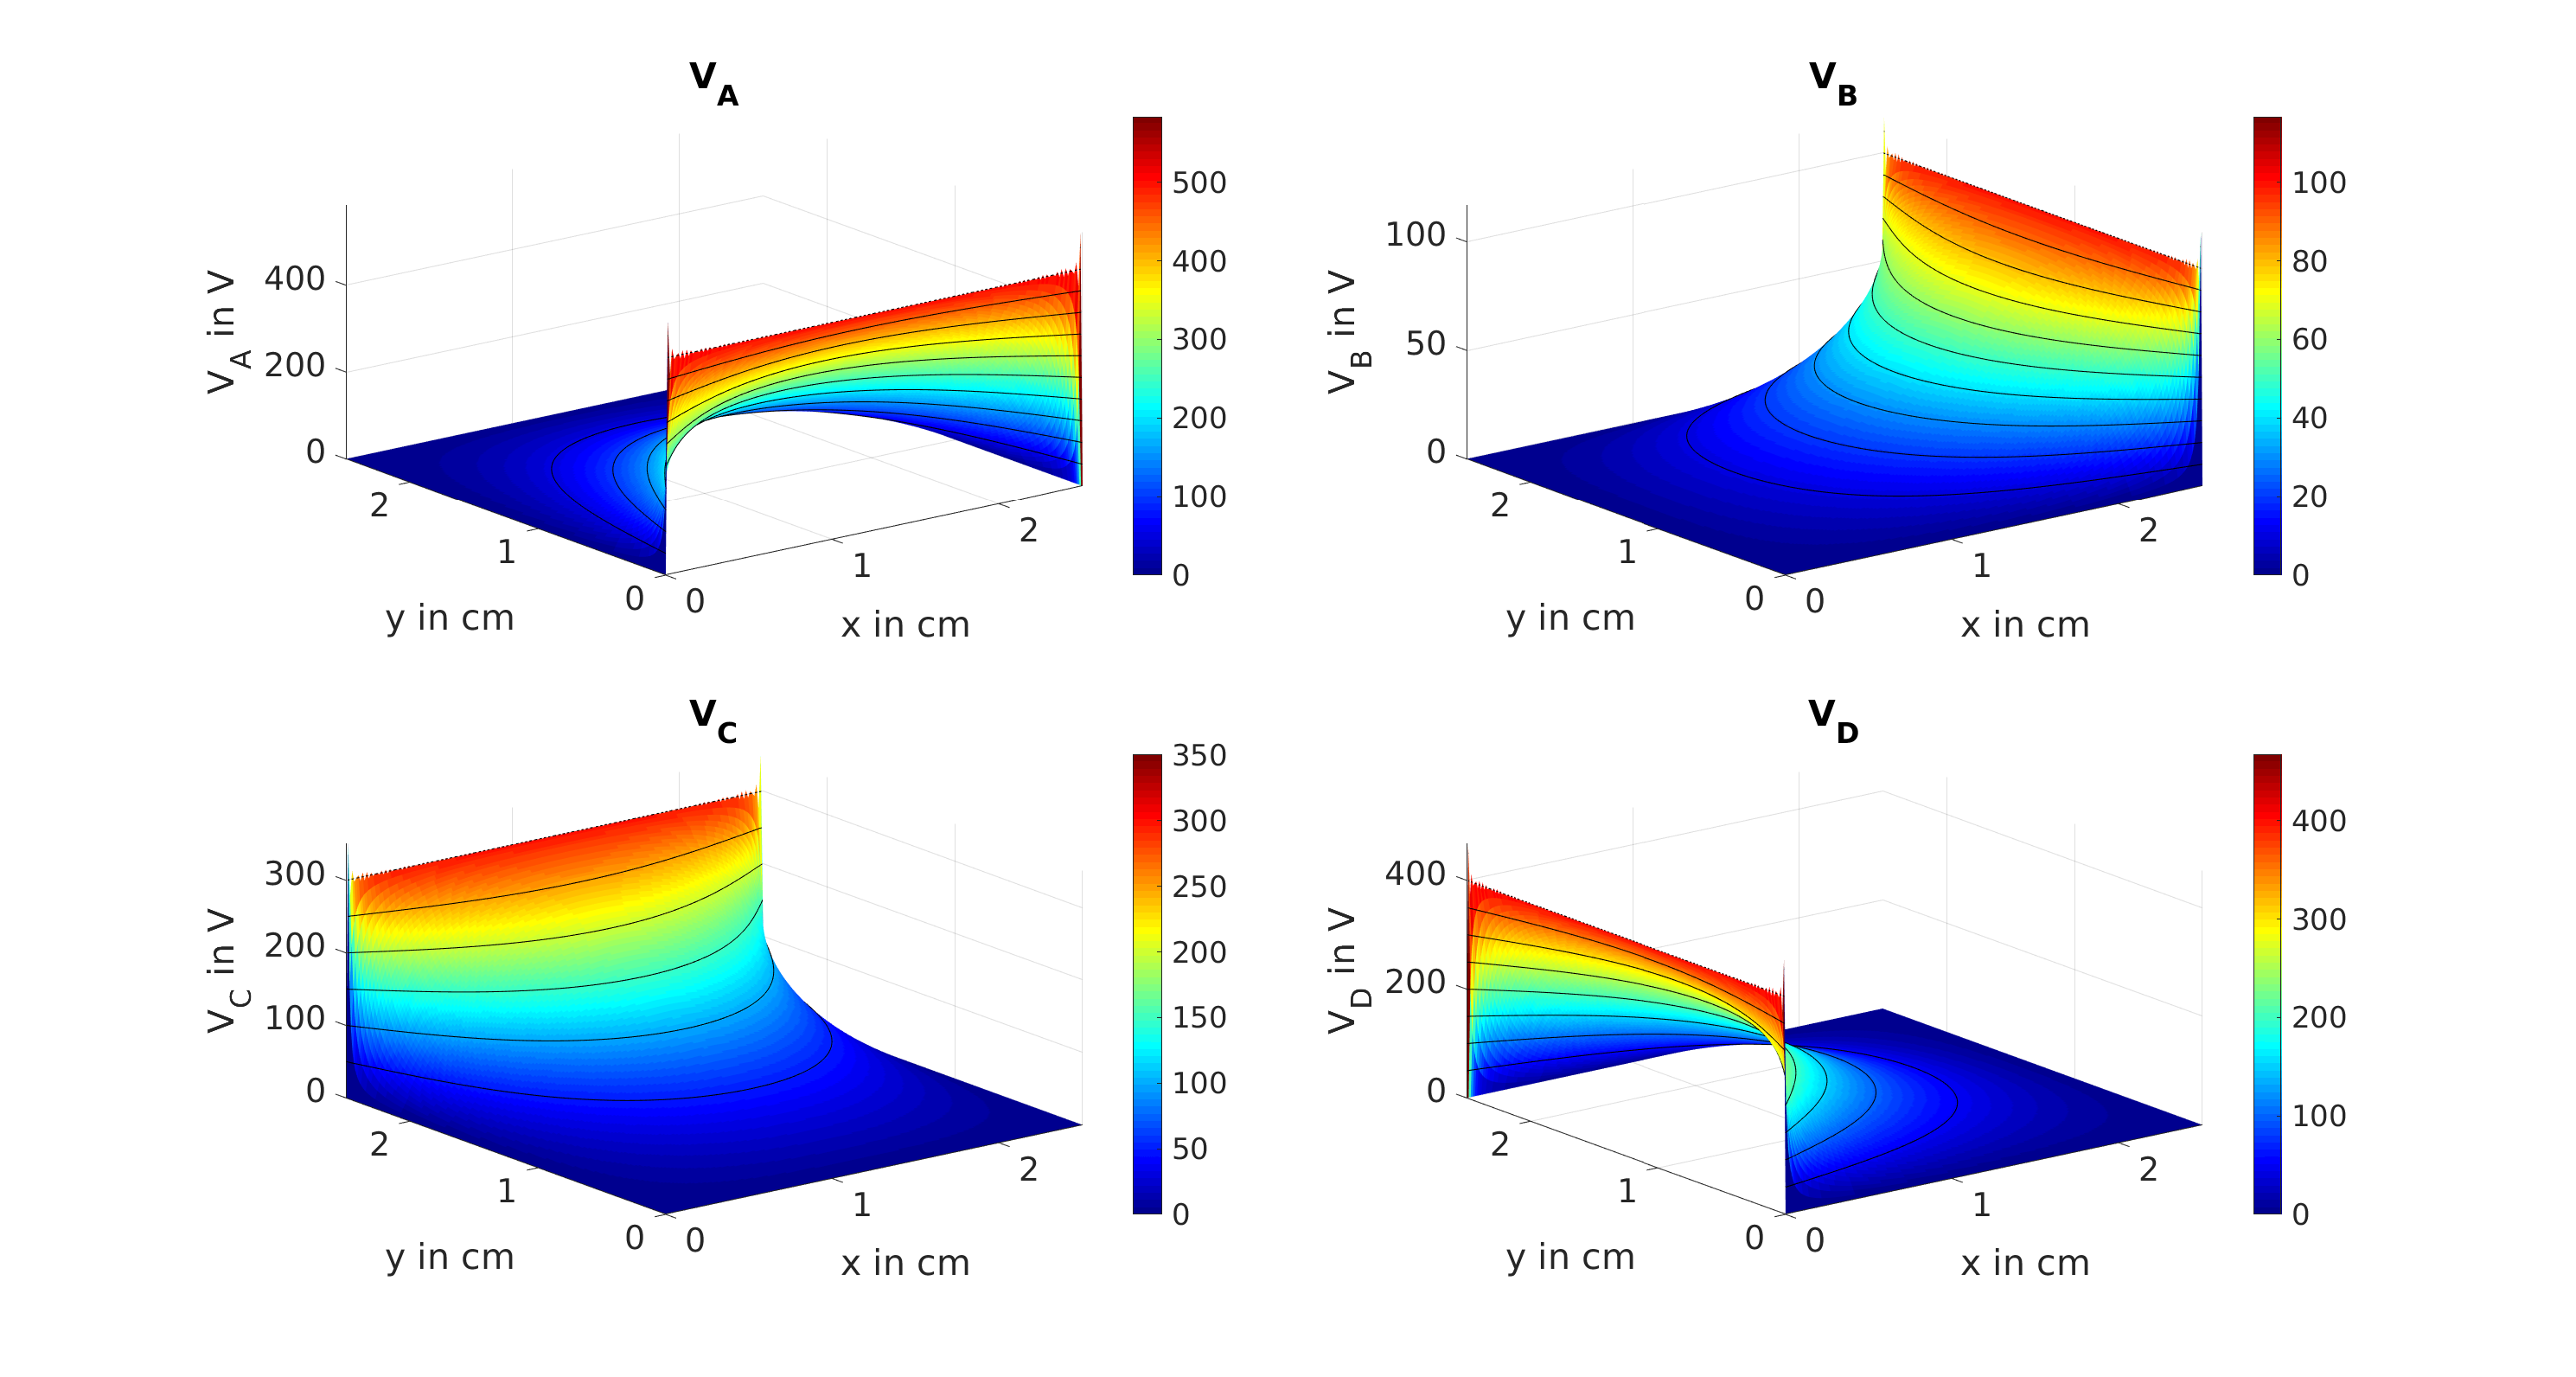
\includegraphics[width=1.0\textwidth]{pics/Bsp_1_analytical_figures/TaskC_fig_1.eps}
  \label{fig:Ana:TaskC:Individual}
  \caption{Potentialverteilung der einzelnen Teillösungen}
\end{figure}

\begin{figure}[H]
  \centering
  		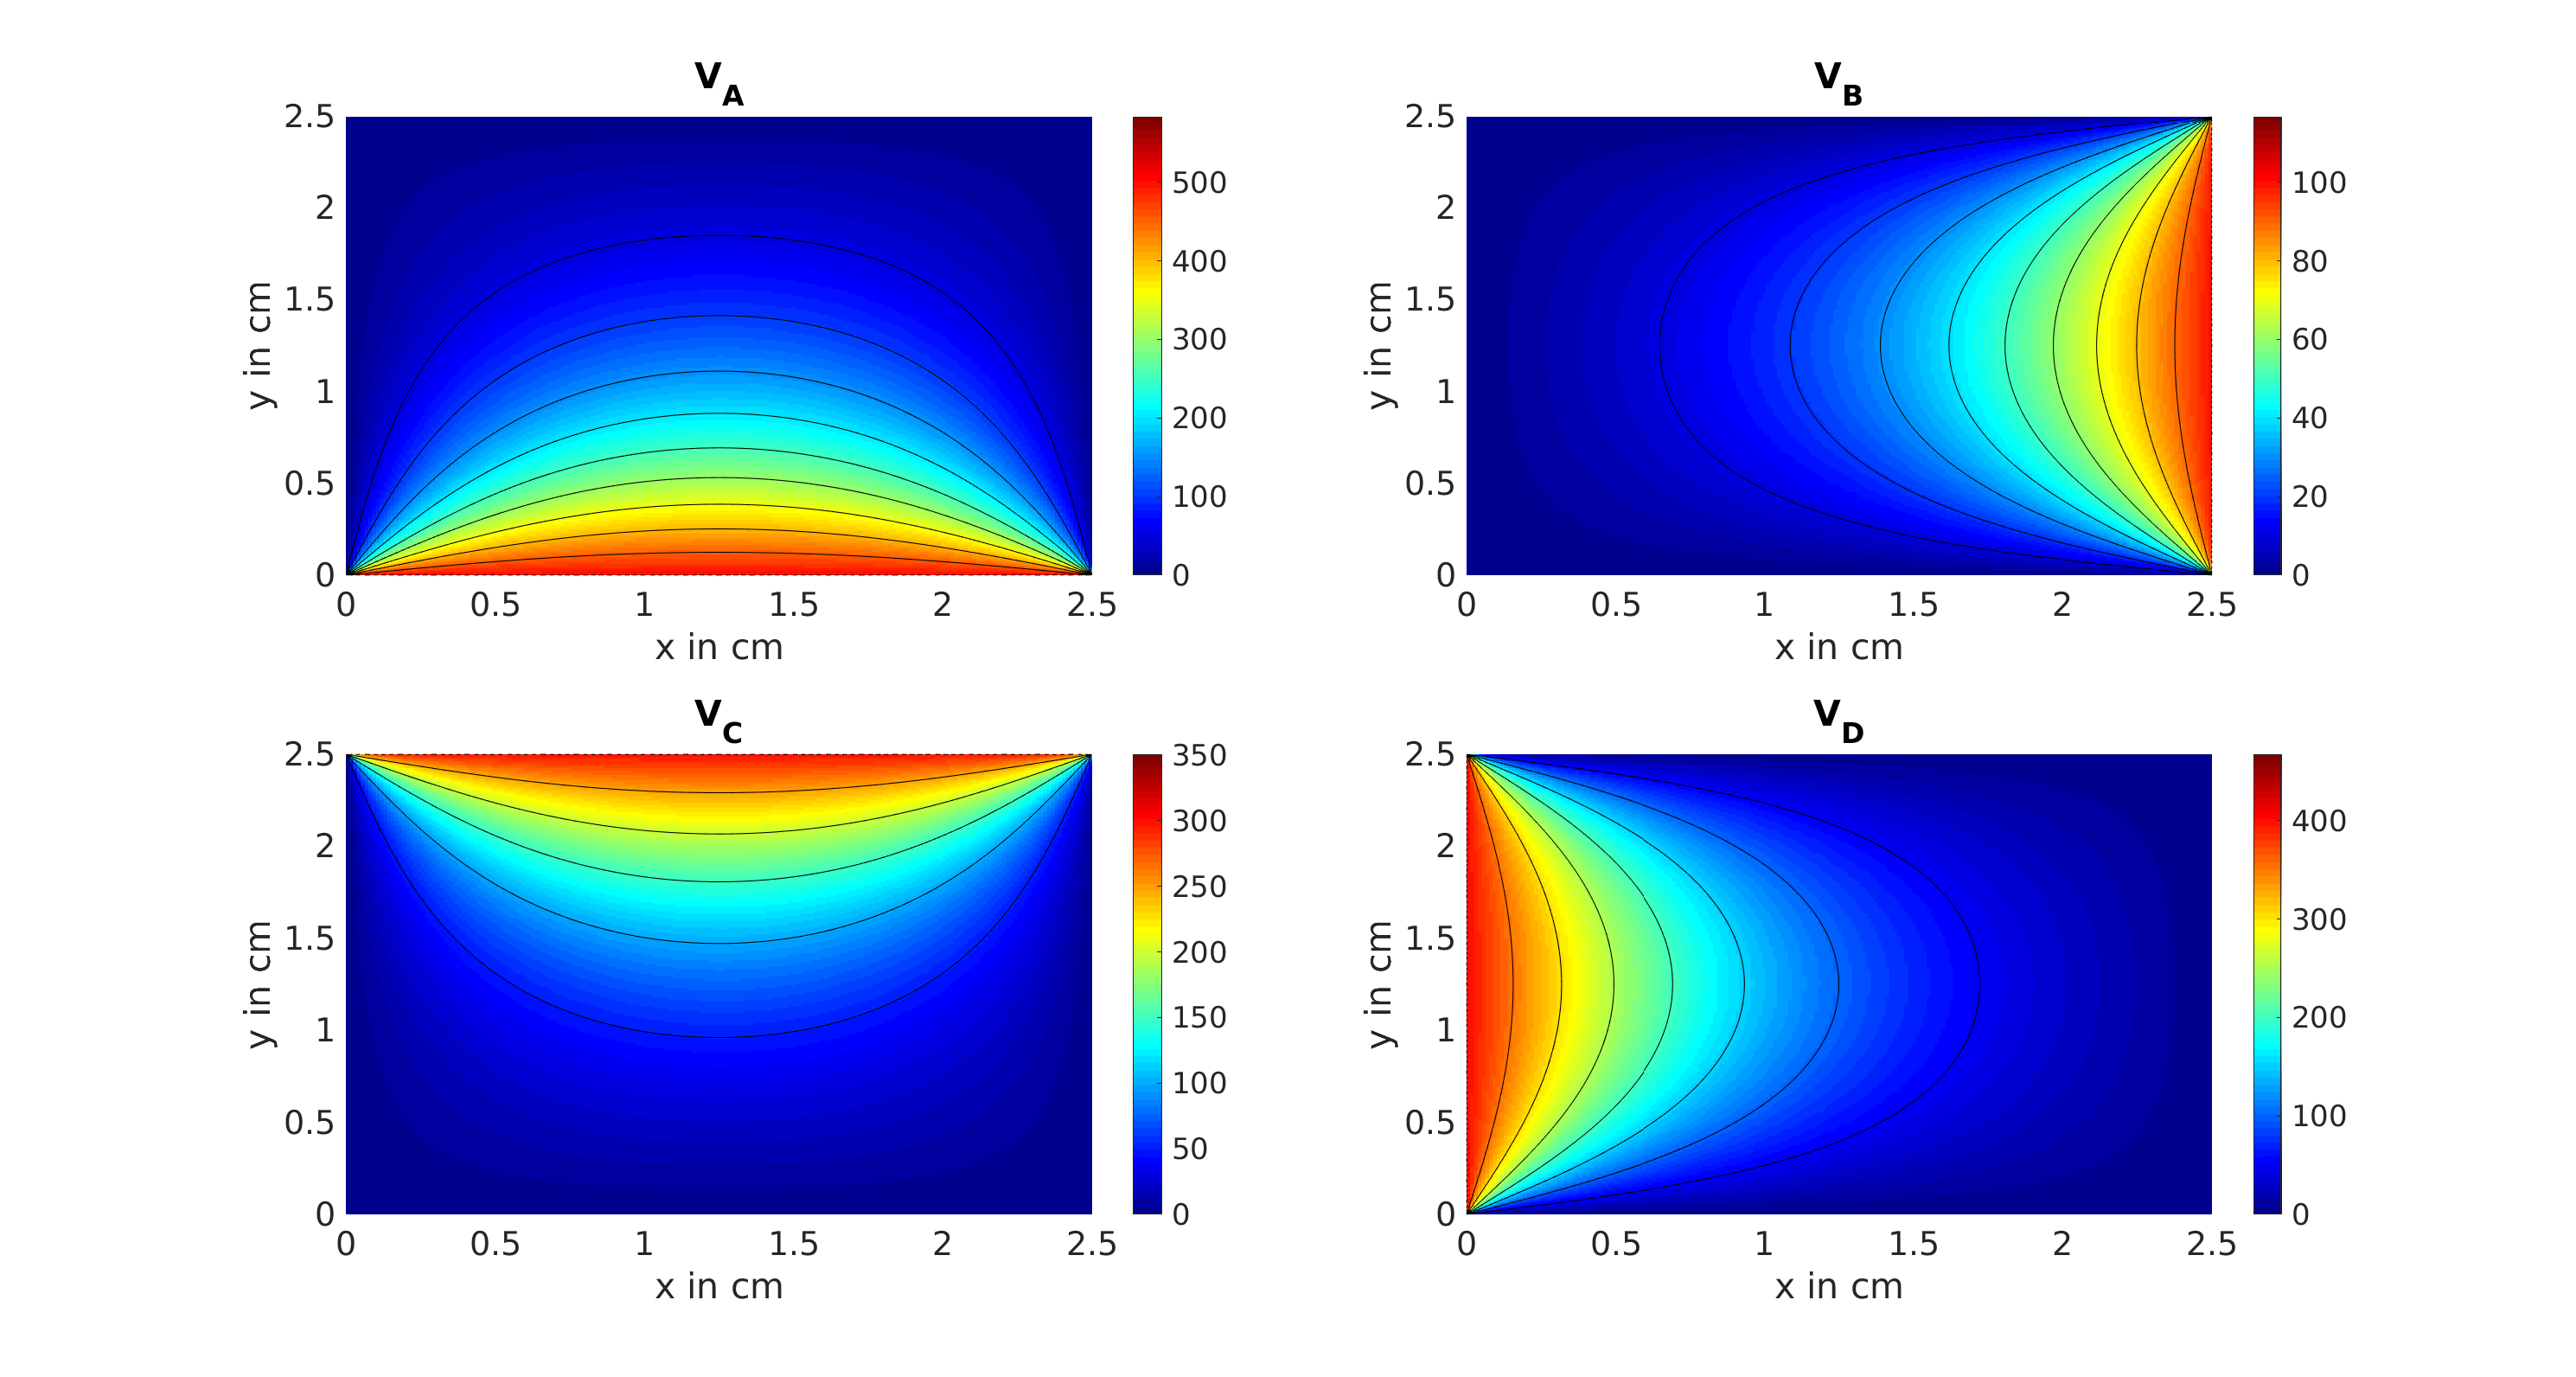
\includegraphics[width=1.0\textwidth]{pics/Bsp_1_analytical_figures/TaskC_fig_3.eps}
  \label{fig:Ana:TaskC:IndividualRot}
  \caption{Potentialverteilung der einzelnen Teillösungen - Draufsicht}
\end{figure}


\newsubsubsection{Gesamtlösung}{}
\begin{figure}[H]
  \centering
  		\includegraphics[width=1.0\textwidth]{pics/Bsp_1_analytical_figures/TaskC_fig_2.eps}
  \label{fig:Ana:TaskC:Complete}
  \caption{Potentialverteilung der Gesamtlösung}
\end{figure}

\begin{figure}[H]
  \centering
  		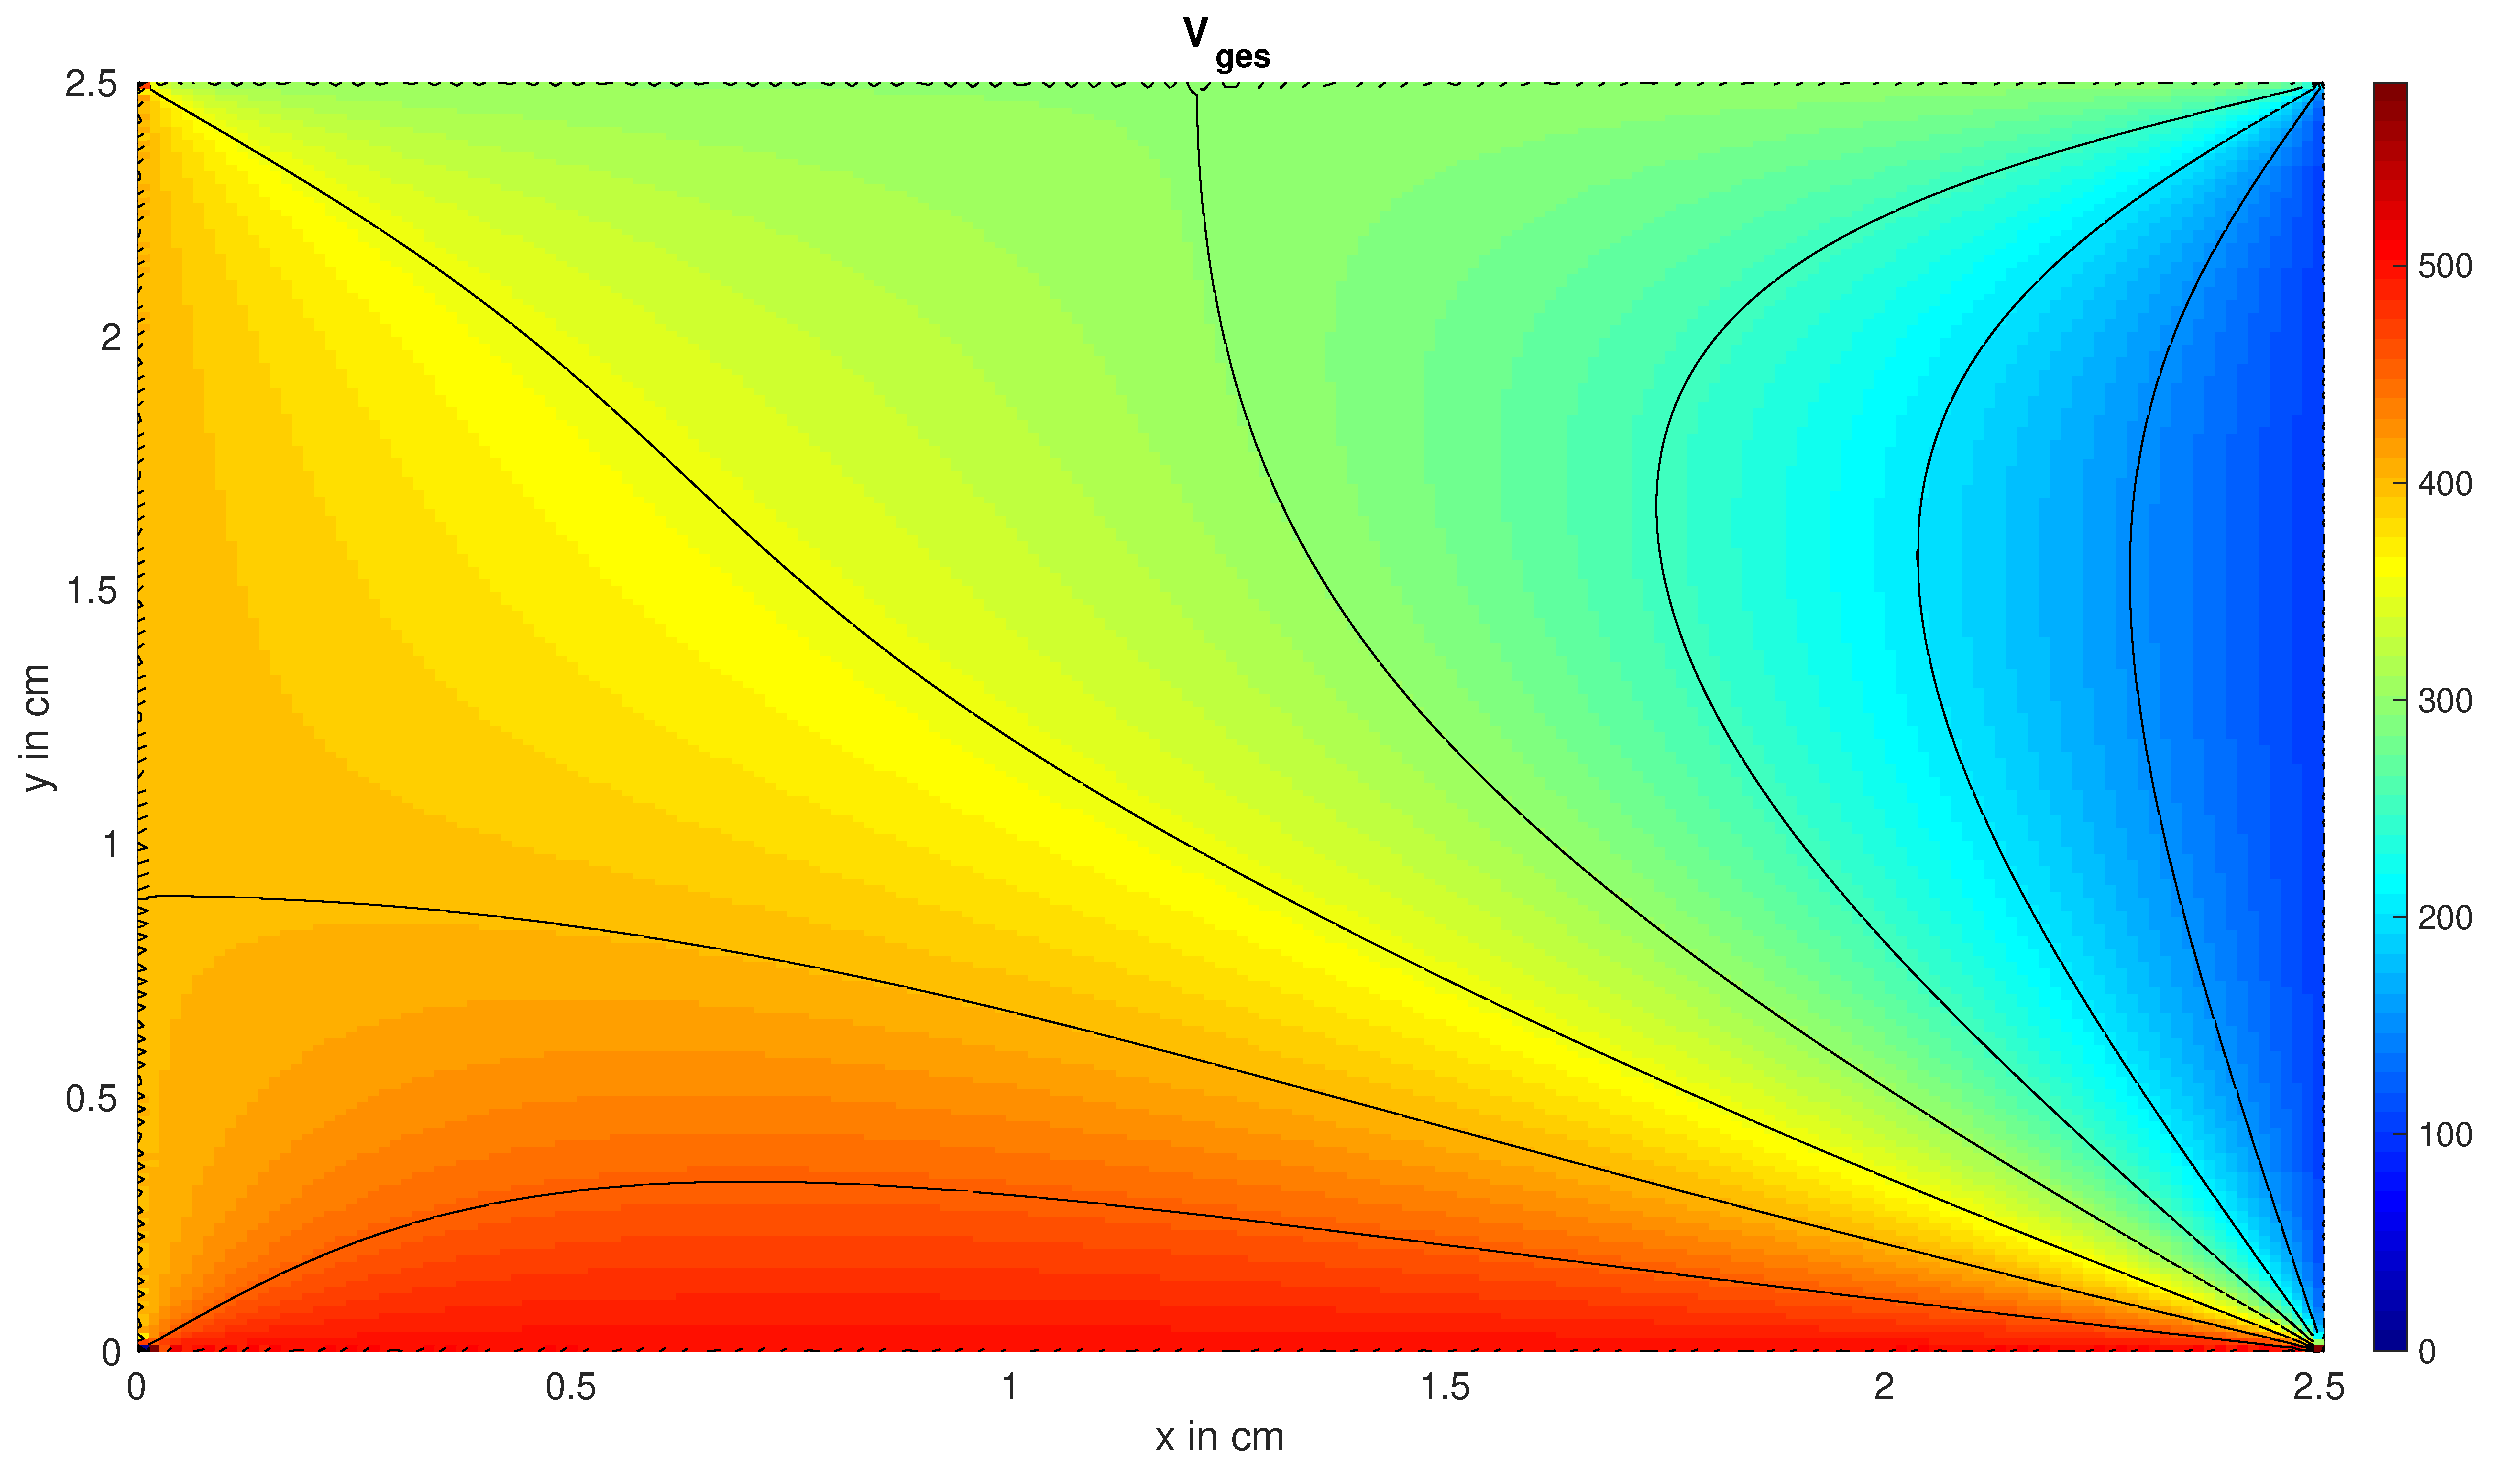
\includegraphics[width=1.0\textwidth]{pics/Bsp_1_analytical_figures/TaskC_fig_4.eps}
  \label{fig:Ana:TaskC:CompleteRot}
  \caption{Potentialverteilung der Gesamtlösung - Draufsicht}
\end{figure}


\newsubsubsection{Feldbild}{}
\begin{figure}[H]
  \centering
  		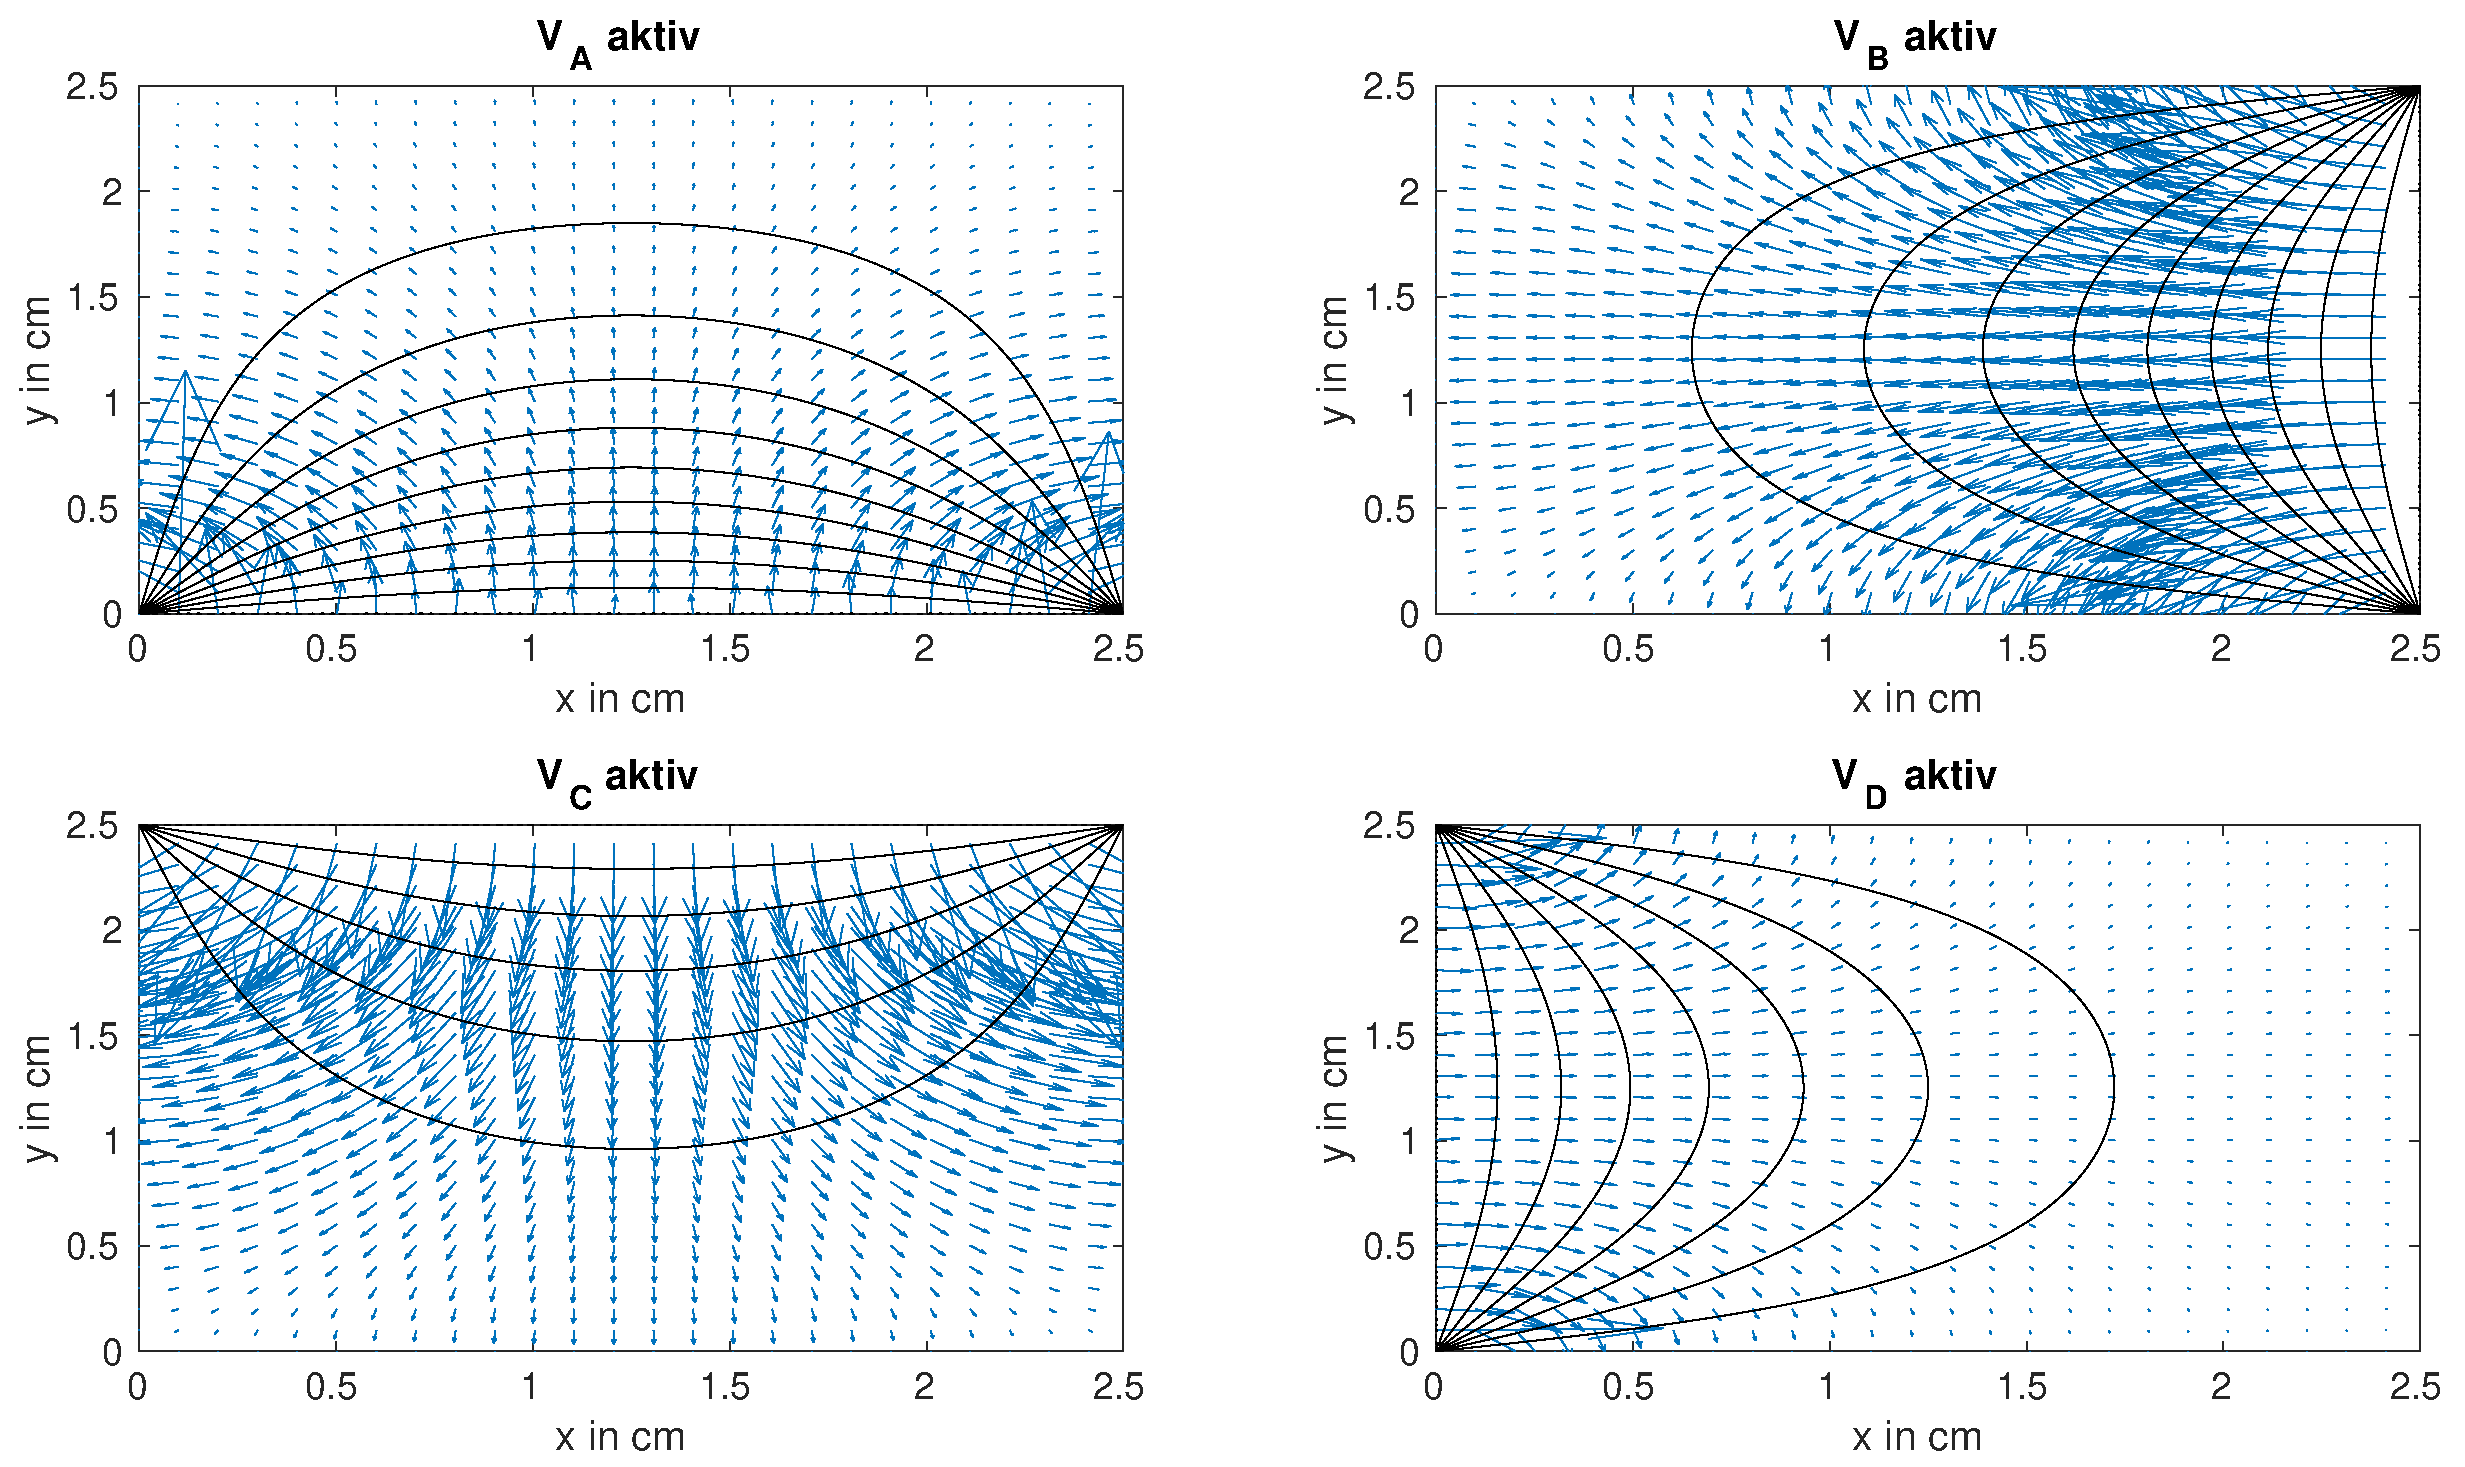
\includegraphics[width=1.0\textwidth]{pics/Bsp_1_analytical_figures/TaskC_fig_5.eps}
  \label{fig:Ana:TaskC:Field:Individual}
  \caption{Feldbild der einzelnen Teillösungen mit Äquipotentiallinien}
\end{figure}

\begin{figure}[H]
  \centering
  		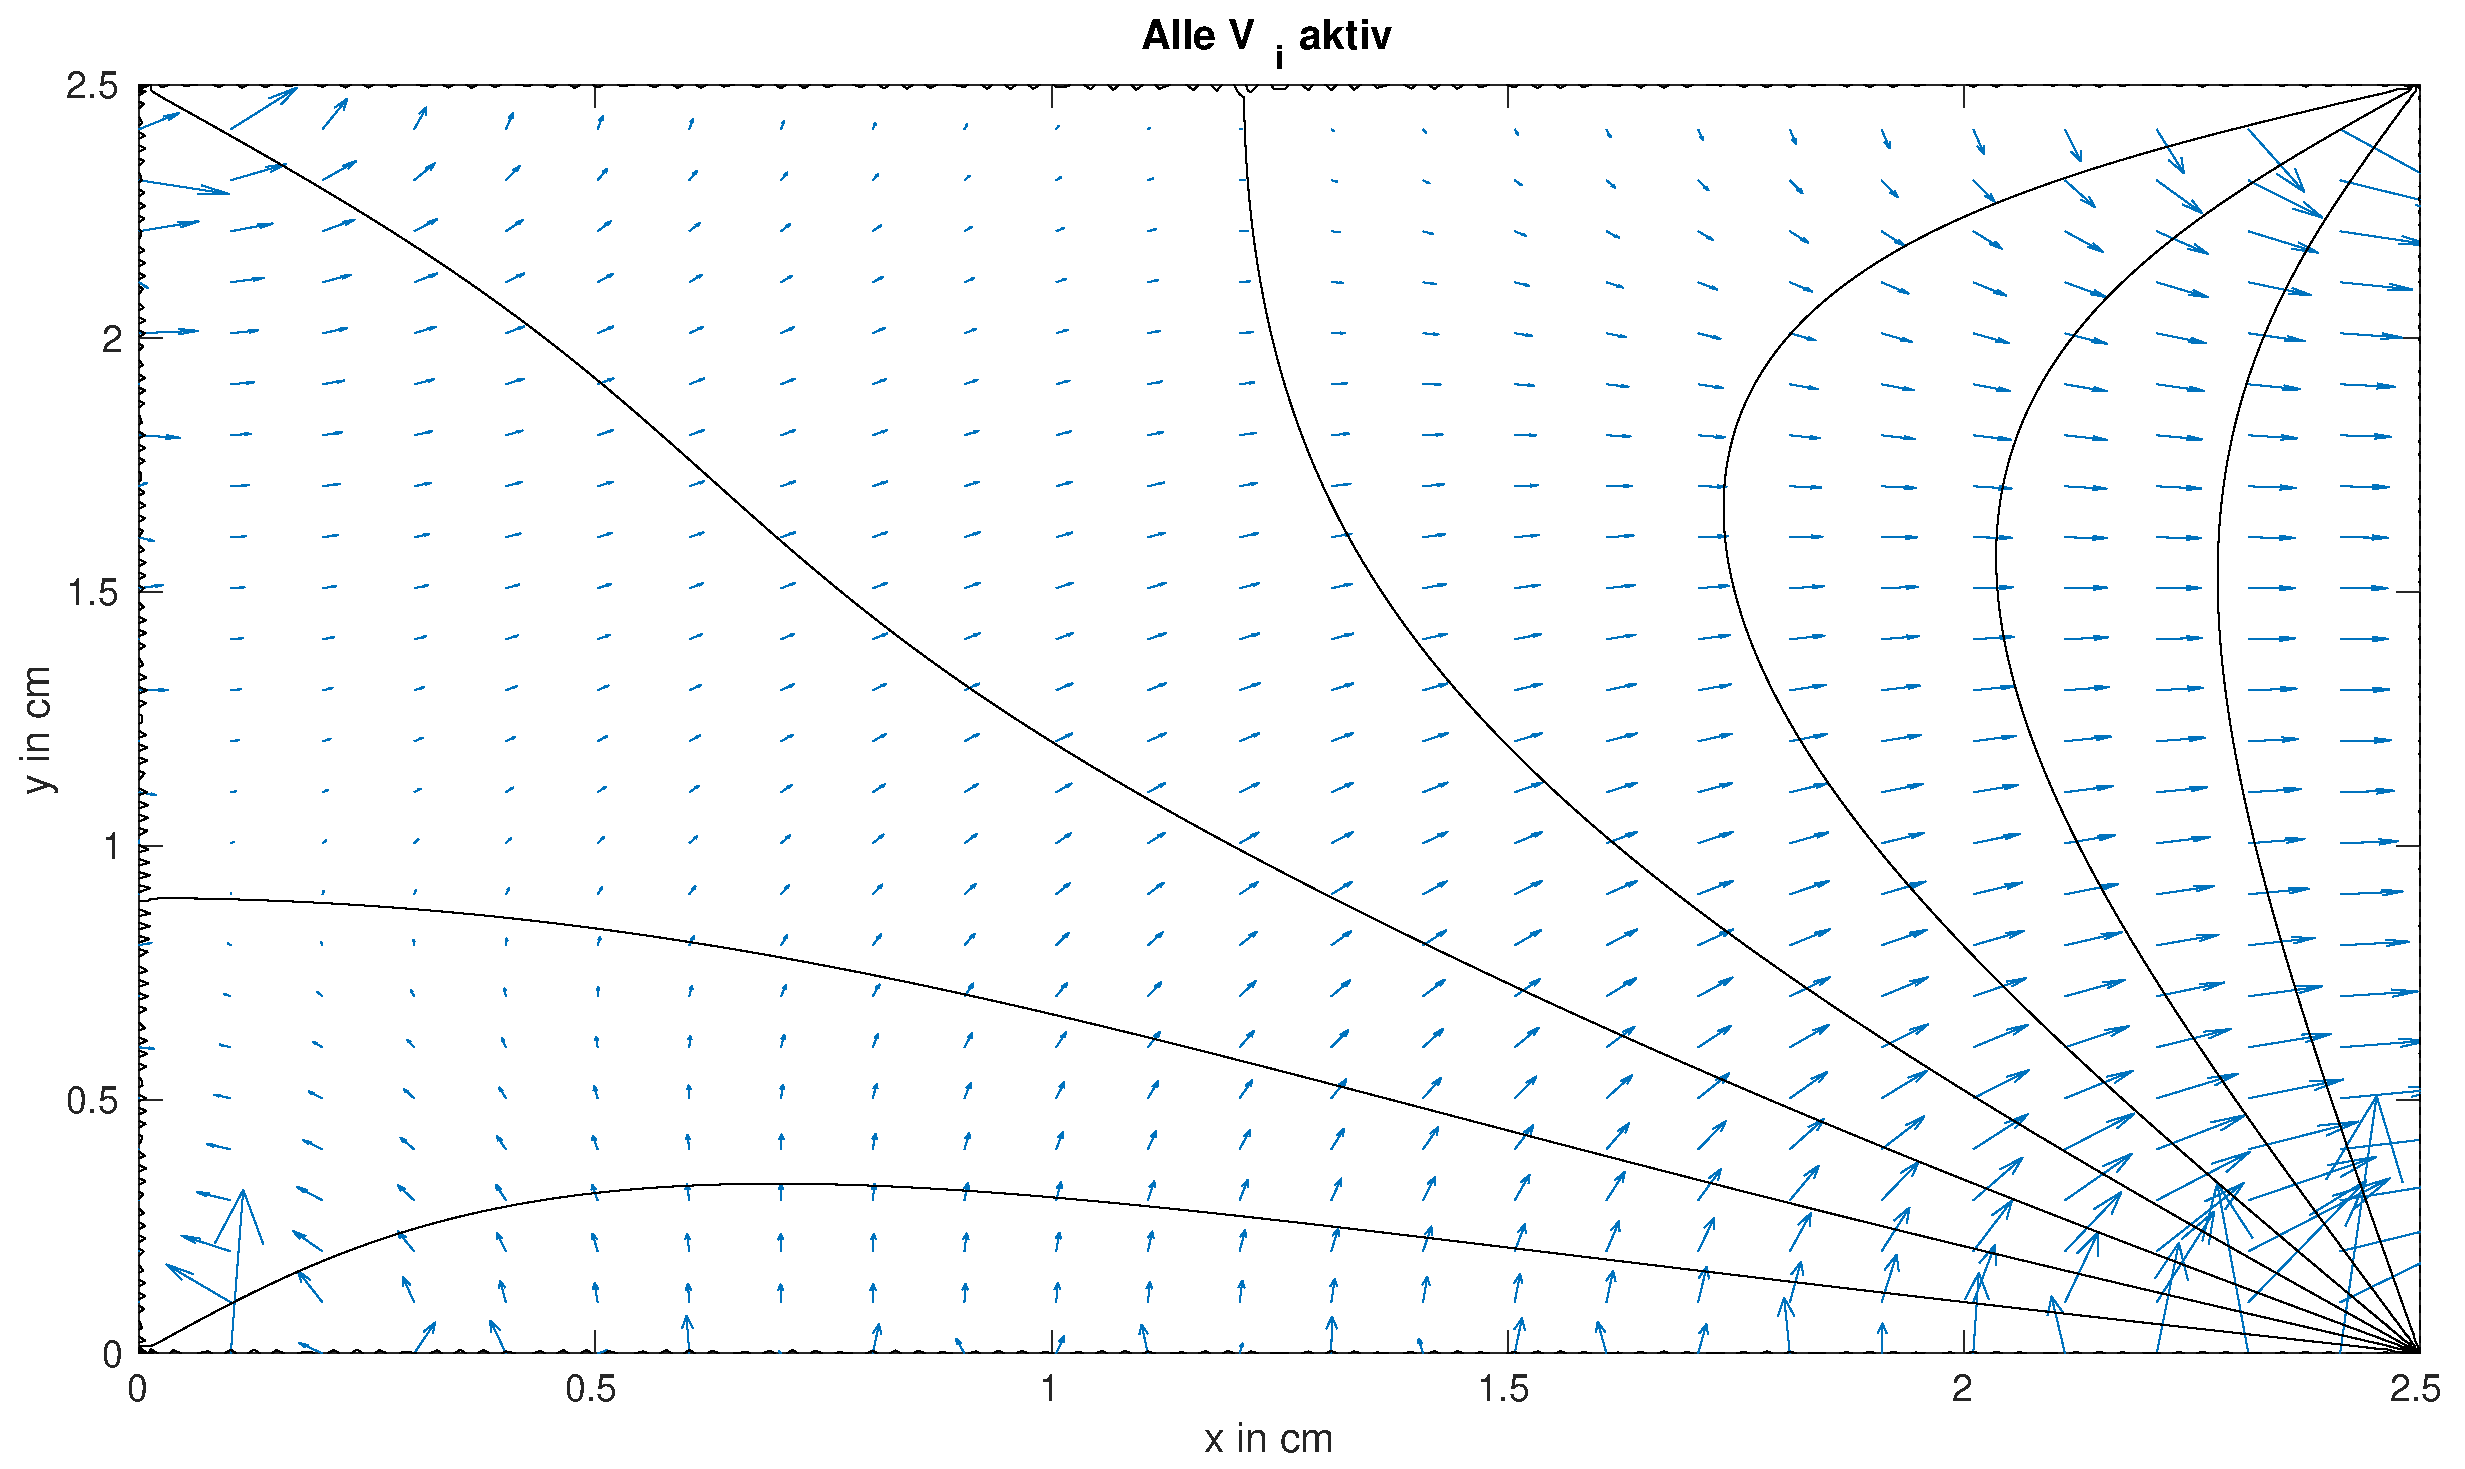
\includegraphics[width=1.0\textwidth]{pics/Bsp_1_analytical_figures/TaskC_fig_6.eps}
  \label{fig:Ana:TaskC:Field:Complete}
  \caption{Feldbild der Gesamtlösung mit Äquipotentiallinien}
\end{figure}

